\documentclass[aoas,preprint]{imsart}\usepackage[]{graphicx}\usepackage[]{xcolor}
% maxwidth is the original width if it is less than linewidth
% otherwise use linewidth (to make sure the graphics do not exceed the margin)
\makeatletter
\def\maxwidth{ %
  \ifdim\Gin@nat@width>\linewidth
    \linewidth
  \else
    \Gin@nat@width
  \fi
}
\makeatother

\definecolor{fgcolor}{rgb}{0.345, 0.345, 0.345}
\newcommand{\hlnum}[1]{\textcolor[rgb]{0.686,0.059,0.569}{#1}}%
\newcommand{\hlsng}[1]{\textcolor[rgb]{0.192,0.494,0.8}{#1}}%
\newcommand{\hlcom}[1]{\textcolor[rgb]{0.678,0.584,0.686}{\textit{#1}}}%
\newcommand{\hlopt}[1]{\textcolor[rgb]{0,0,0}{#1}}%
\newcommand{\hldef}[1]{\textcolor[rgb]{0.345,0.345,0.345}{#1}}%
\newcommand{\hlkwa}[1]{\textcolor[rgb]{0.161,0.373,0.58}{\textbf{#1}}}%
\newcommand{\hlkwb}[1]{\textcolor[rgb]{0.69,0.353,0.396}{#1}}%
\newcommand{\hlkwc}[1]{\textcolor[rgb]{0.333,0.667,0.333}{#1}}%
\newcommand{\hlkwd}[1]{\textcolor[rgb]{0.737,0.353,0.396}{\textbf{#1}}}%
\let\hlipl\hlkwb

\usepackage{framed}
\makeatletter
\newenvironment{kframe}{%
 \def\at@end@of@kframe{}%
 \ifinner\ifhmode%
  \def\at@end@of@kframe{\end{minipage}}%
  \begin{minipage}{\columnwidth}%
 \fi\fi%
 \def\FrameCommand##1{\hskip\@totalleftmargin \hskip-\fboxsep
 \colorbox{shadecolor}{##1}\hskip-\fboxsep
     % There is no \\@totalrightmargin, so:
     \hskip-\linewidth \hskip-\@totalleftmargin \hskip\columnwidth}%
 \MakeFramed {\advance\hsize-\width
   \@totalleftmargin\z@ \linewidth\hsize
   \@setminipage}}%
 {\par\unskip\endMakeFramed%
 \at@end@of@kframe}
\makeatother

\definecolor{shadecolor}{rgb}{.97, .97, .97}
\definecolor{messagecolor}{rgb}{0, 0, 0}
\definecolor{warningcolor}{rgb}{1, 0, 1}
\definecolor{errorcolor}{rgb}{1, 0, 0}
\newenvironment{knitrout}{}{} % an empty environment to be redefined in TeX

\usepackage{alltt}
\usepackage{amsmath}
\usepackage{amssymb}
\usepackage{graphicx}
\usepackage{subcaption}
\usepackage{enumerate}
\usepackage[authoryear]{natbib}
\usepackage{graphicx}
\usepackage[english]{babel}
\usepackage[colorlinks=true, allcolors=blue]{hyperref}
\usepackage{caption}
\usepackage{subcaption}
\usepackage{placeins}
\usepackage{booktabs}
\usepackage{tabularx}
\usepackage[ruled]{algorithm2e}
\usepackage{hyperref}
\usepackage{float}
\usepackage[utf8]{inputenc}
\usepackage{hyphenat}
\tolerance=1000
\usepackage{url}
\usepackage{makecell}
\usepackage{textcomp}
\usepackage{tikz}
\usepackage{hyphenat}
\usepackage{tikz}
\usetikzlibrary{arrows.meta, shapes.geometric, positioning}
\bibliographystyle{apalike}
\newcommand{\blind}{1}

\newcommand\Unit{U}
\newcommand\unit{u}
\newcommand\seq[2]{{#1}\!:\!{#2}}
\newcommand\species{\mathbbm{k}}
\newcommand\params{\, ; \,}
\usepackage{bbm}
\newcommand\native{\mathbbm{n}}
\newcommand\invasive{\mathbbm{i}}
\newcommand\Normal{\mathrm{N}}
\newcommand\benchmarktime{n}

\parskip 3mm
\newcommand\authoraddress{ \vspace{-1mm} \\ \normalsize}
\newcommand\jwc[1]{\textcolor{brown}{[JW: #1]}}
\newcommand\eic[1]{\textcolor{orange}{[EI: #1]}}
\newcommand\byc[1]{\textcolor{blue}{[BY: #1]}}
\newcommand\TODO[1]{\textcolor{red}{[TODO: #1]}}

\renewcommand{\contentsname}{Supplementary Content}
\renewcommand{\refname}{Supplementary References}
\renewcommand\thefigure{S-\arabic{figure}}
\renewcommand\thetable{S-\arabic{table}}
%\renewcommand\thepage{S-\arabic{page}}
\renewcommand\thesection{S\arabic{section}}
\renewcommand\theequation{S\arabic{equation}}
\renewcommand\thealgocf{S\arabic{algocf}}
\setcounter{tocdepth}{2}
\IfFileExists{upquote.sty}{\usepackage{upquote}}{}
\begin{document}





\begin{frontmatter}
\title{Supplement to ``Mechanistic models for panel data: Analysis of ecological experiments with four interacting species''}

\if1\blind
{
\begin{aug}
\author[A]{\fnms{Bo}~\snm{Yang}\ead[label=e1]{ybb@umich.edu}},
\author[B]{\fnms{Jesse}~\snm{Wheeler}\ead[label=e2]{jeswheel@umich.edu}},
\author[C]{\fnms{Meghan A.}~\snm{Duffy}\ead[label=e3]{duffymeg@umich.edu}},
\author[C]{\fnms{Aaron A.}~\snm{King}\ead[label=e4]{kingaa@umich.edu}}
\and
\author[D]{\fnms{Edward}~\snm{Ionides}\ead[label=e5]{ionides@umich.edu}}

\address[A]{Department of Marketing, Columbia University \printead[presep={,\ }]{e1}}
\address[B]{Department of Mathematics and Statistics, Idaho State University\printead[presep={,\ }]{e2}}
\address[C]{Department of Ecology and Evolutionary Biology, University of Michigan
\address[D]{Department of Statistics, University of Michigan\printead[presep={,\ }]{e5}}
 \printead[presep={,\ }]{e3,e4}}
\end{aug}
} \fi
\end{frontmatter}



\tableofcontents
\newpage
\section{Monte Carlo Adjusted Profile}

Monte Carlo Adjusted Profile (MCAP) methods \citep{ionides17,ning21} provide confidence intervals for situations where the likelihood is evaluated and maximized by Monte Carlo algorithms.
A smoothed estimate of the profile likelihood is used to reduce Monte Carlo error, quantify this error, and adjust the confidence intervals accordingly to maintain their coverage.

\parskip 3mm

MCAP is particularly useful for high-dimensional situations, such as arise in panel data analysis, since it becomes practically impossible to apply sufficient computational effort to make Monte Carlo error negligible.
MCAP has previously been demonstrated for panel iterated filtering by \citet{breto20}.

\parskip 3mm

To investigate identifiability, we carried out an additional exploration to obtain estimates, profiles and confidence intervals for the composite parameters,  $r^{\species}f^{\species}_{S}$ and $r^{\species}f^{\species}_{S}$, as well as the individual parameters.
We could have reparameterized to apply MCAP to these composite parameters exactly as we did for the individual parameters.
However, for this additional analysis we made a simplification by re-using the calculations for the original profiles.
For every point on every profile, computed for the individual parameters, we calculated the value of the composite parameters.
We obtained the highest log-likelihoods within a grid of values for the composite parameters and applied MCAP to these values.
We have found previously that these ``poor man's profiles'' provide a reasonable approximation to the true profile, while avoiding the need to work with a reparameterized version of the model.
We calculated these composite parameters only for the SIRJPF2 model, and the results are shown together with the individual parameters, in Table~1 and Figure~S-1.

\section{The Panel Iterated Filtering Algorithm}

\begin{algorithm}[h]
\caption{Panel iterated filter (PIF)}
\label{alg:pif}
\DontPrintSemicolon
\KwIn{PanelPOMP model, as defined in Section~3 of the main text\;
  Number of particles, $J$, and filter iterations, $M$\;
  Cooling factor $\rho$\;
  Starting parameter vector swarm, \( \Theta^{(0)}_{j} = (\Phi^{(0)}_{j},\Psi^{(0)}_{1:U,j}) \),
  for $j = \seq{1}{J}$\;
  Perturbation variance, $V^\Theta_{u,n}$, for $u=\seq{1}{U}$, $n=\seq{1}{N_u}$\;
  Logical variable determining marginalization, $\mathrm{MARGINALIZE}$
  }
\KwOut{Parameter swarm, $\Theta^{(M)}_{1:J}$, approximating the MLE}
\For{\( m = 1 \) \KwTo \( M \)}{
  $\Theta^{F,m}_{0,j} = \Theta^{(m-1)}_{j}$ for $j = \seq{1}{J}$\;
  \For{\( u = 1 \) \KwTo \( U \)}{
    $(\Phi^{F,m}_{u,0,j},\Psi^{F,m}_{u,0,j}) \sim \mathcal{N}(\Theta^{F,m}_{u-1,j},\rho^{2m}V^\Theta_{u,0})$ for $j = \seq{1}{J}$\;
    \( X_{u,0,j}^{F,m} \sim f_{X_{u,0}}(\, \cdot \params \Phi^{F,m}_{u,0,j},\Psi^{F,m}_{u,0,j}) \) for $j = \seq{1}{J}$\;
    \For{\( n = 1 \) \KwTo \( N_u \)}{
       $\Phi^{P,m}_{u,n,j} \sim \mathcal{N}\big(\Phi^{F,m}_{u,n-1,j}, \rho^{2m}V^\Phi_{u,n}\big)$ for $j = \seq{1}{J}$\;
       $\Psi^{P,m}_{u,n,j} \sim \mathcal{N}\big(\Psi^{F,m}_{u,n-1,j}, \rho^{2m}V^\Psi_{u,n}\big)$ for $j = \seq{1}{J}$\;
       \( X_{u,n,j}^{P,m} \sim f_{X_{u,n} | X_{u,n-1}}\big(\, \cdot \mid X_{u,n-1,j}^{F,m} \params \Phi^{P,m}_{u,n,j},\Psi^{P.m}_{u,n,j}\big) \) for \( j = \seq{1}{J} \)\;
       $w_{u,n,j}^m = f_{Y_{u,n} | X_{u,n}}\big(y^*_{u,n} \mid X^{F,m}_{u,n,j} \params \Phi^{P,m}_{u,n,j},\Psi^{P.m}_{u,n,j}\big)$ for \( j = \seq{1}{J} \)\;
       $k_j = i$ with probability proportional to $ w_{u,n,i}^m$ for $i,j = \seq{1}{J}$\;
       $X^{F,m}_{u,n,j} = X^{P,m}_{u,n,k_j}$ for $j = \seq{1}{J}$\;
       $\Phi^{F,m}_{u,n,j} = \Phi^{P,m}_{u,n,k_j}$ for $j = \seq{1}{J}$\;
       $\Psi^{F,m}_{u,n,j} = \Psi^{P,m}_{u,n,k_j}$ for $j = \seq{1}{J}$\;
              \uIf{$\mathrm{MARGINALIZE}$}{$\Psi^{F,m}_{\tilde u,n,j} = \Psi^{P,m}_{\tilde u,n,j}$ for all $\tilde u \neq u$, $j=\seq{1}{J}$}
       \Else{$\Psi^{F,m}_{\tilde u,n,j} = \Psi^{P,m}_{\tilde u,n,k_j}$ for all $\tilde u \neq u$, $j=\seq{1}{J}$}
       }
  $\Theta^{F,m}_{u,j} = \big( \Phi^{F,m}_{u,N_u,j},  \Psi^{F,m}_{1:U,N_u,j} \big)$
  }
  $\Theta^{(m)}_{j} = \Theta^{F,m}_{U,j}$;
}
\end{algorithm}

Algorithm~\ref{alg:pif} presents pseudocode for PIF.
Here, $\Phi^{F,m}_{u,n,j}$ is the $j$th filter particle searching for the MLE of the shared parameter $\phi$ in the $m$th filter iteration, at time point $n$ and unit $u$.
 $\Psi^{F,m}_{u,n,j}$ is the corresponding quantity searching for the MLE of the unit-specific parameter, $\psi_u$.
Cooling factor $\rho$ determines how aggressively the parameter perturbations are dampened as the number of iterations increases.
By gradually reducing the size of these parameter random walks, the algorithm refines the parameter estimates and converges more tightly to the maximum likelihood point.

When $\mathrm{MARGINALIZE}=\mathrm{TRUE}$, the estimate of the unit-specific parameter $\psi_u$ belonging to particle $j$ is unchanged when filtering throuth a unit $\tilde u\neq u$. 
The unmarginalized PIF was proposed by \cite{breto20} and was provided with theoretical convergence results that are not yet available for MPIF.
However, our results demonstrate that MPIF has superior empirical performance on the ecological model considered here.
Theoretical support for MPIF will be published elsewhere \citep{wheeler25}.

To briefly review, the model is specified by the initial condition, $ f_{X_{u,0}}(\, \cdot \, \params \phi,\psi_u)$, the latent state transition density, $f_{X_{u,n} | X_{u,n-1}}\big(\, \cdot \mid \,  \params \phi,\psi_u \big)$, and the measurement density, $f_{Y_{u,n} | X_{u,n}}\big(\, \cdot \mid \cdot \params \phi,\psi_u\big)$, for $u = \seq{1}{U}$ and $n=\seq{1}{N_u}$.
The full parameter vector is written as $\theta=(\phi,\psi_{1:U})$.
For notational convenience, we define $u=0$ to be an empty panel with $N_0=0$.
Algorithm~\ref{alg:pif} supposes Gaussian perturbations of the parameters, which is a common practical choice but may require re-parameterizing to avoid boundaries.
For example, non-negative parameters are typically log-transformed.
Additional generality is provided by the pseudocode in \cite{breto25} that is implemented in the \texttt{mif2} function of the R package \texttt{panelPomp}.

\clearpage

\section{SIRJPF2 Model}
\subsection{Results}
\begin{figure}[!ht]
    \centering
    \includegraphics[width=\linewidth]{profile/Target_dynamics/para/Profile_plot.png}
    \caption{Monte Carlo Adjusted Profile results of SIRJPF2 model for mixed species Parasitized dynamics.
    The vertical dotted lines represent the 95\% confidence interval obtained by MCAP.
    The vertical blue lines show the MLE estimated using MCAP.
    The red vertical lines correspond to the model with the overall highest likelihood among all searches. }
    \label{fig:SIRJPF2_profile}
\end{figure}


In the panelPOMP framework, one must decide whether or not each parameter should be unit specific, or shared across units.
These decisions greatly affect the degree of freedom for each model. For example, with ten units in the model, adding a shared parameter increases the model’s dimension by one, and adding a unit specific parameter will increase the dimension by ten.
An increase in parameter dimension increases the model’s ability to quantitatively describe the observed data, but leads to the possibility of over-fitting, resulting in a model with poor explanatory and predictive power.
In order to find a balance between fitting accuracy and simplicity when selecting models, we employed the Akaike information criterion (AIC) as a criteria to compare models while adjusting for dimension.
We estimate model parameters via maximum likelihood using the panel iterated filtering (PIF) \citep{breto20} and calculate AIC for all models.
In addition to AIC, we report $p$-values from the likelihood ratio test (LRT) to provide a complementary assessment of whether unit-specific parameterizations yield a statistically significant improvement in model fit over the all-shared baseline.
The LRT compares each unit-specific model (alternative) against the all-shared model (null) as a nested pair: the all-shared model is the restricted case obtained by constraining all unit-specific copies of a parameter to be equal.
The test statistic $\Lambda = 2[\ell(\text{alternative}) - \ell(\text{null})]$ is referred to a $\chi^2$ distribution with degrees of freedom equal to the difference in the number of estimated parameters between the two models.
Since the log-likelihoods in our framework are evaluated via Monte Carlo methods, both the AIC values and LRT $p$-values are subject to Monte Carlo variability, and we interpret them accordingly.
The following table shows the comparison of different models under different settings of unit specific parameter.
Each row represents a different model configuration, with specific parameters designated as either unit-specific or shared across all units.
Within the table, the max log-likelihood and AIC columns report the maximum log-likelihood and AIC values for each model configuration, where a lower AIC indicates a more favorable balance between model fit and complexity. Similarly, the max log-likelihood (MPIF) and AIC (MPIF) columns provide analogous metrics under the marginalized method setting for the PIF procedure. The LRT $p$-value column reports the $p$-value from the likelihood ratio test of each unit-specific model against the all-shared baseline, with ``---'' denoting the reference model.
\begin{table}[h!]
\centering
\small
\begin{center}
\begin{tabular}{||c |c |c |c|c|c||}
 \hline
Specific parameters  & Max log-likelihood & AIC & \makecell[c]{Max log-likelihood\\(MPIF)} & \makecell[c]{AIC\\(MPIF)} & \makecell[c]{LRT\\$p$-value}\\ [0.5ex]
 \hline\hline
$\varnothing$ & -880.56& 1809.12& -880.56& 1809.12 & --- \\
$\theta^{\species}_{I,\unit}$ & -867.76& 1811.51& -863.03& 1802.05 & 0.03 \\
$p^{\species}_{\unit}$ & -868.04& 1812.07& -865.80& 1807.61 & 0.03 \\
$\theta_{P,\unit}$ & -878.32& 1818.64& -875.87& 1813.75 & 0.72 \\
$\xi_{\unit}$ & -880.84& 1823.67& -879.24& 1820.48 & $>$0.99 \\
$\theta^{\species}_{S,\unit}$ & -881.09& 1838.18& -872.08& 1820.17 & $>$0.99 \\
$f^{\species}_{S,\unit}$ & -881.53& 1839.05& -872.49& 1820.99 & $>$0.99 \\
$r^{\species}_{\unit}$ & -883.93& 1843.87& -870.46& 1816.93 & $>$0.99 \\[1ex]
 \hline
\end{tabular}
\end{center}
\caption{Comparison of model fit and complexity across various configurations of unit-specific parameters within the panelPOMP framework for mixed species Parasitized dynamics. The unit-specific parameter setting assessed include ($\theta^{\species}_{I,\unit}$), ($p^{\species}_{\unit}$), $\xi_{\unit}$, ($f^{\species}_{S,\unit}$ ), ($\theta^{\species}_{S,\unit}$), $\theta_{P,\unit}$ and ($r^{\species}_{\unit}$) for $\species \in \{\native,\invasive\}$.}
\label{Table:SIRJPF2_model_comparison}
\end{table}

Table~\ref{Table:SIRJPF2_model_comparison} shows that the all-shared-parameters model ($\varnothing$) achieves the lowest AIC among all configurations considered.
The LRT $p$-values indicate that none of the unit-specific parameterizations yield a statistically significant improvement over the all-shared baseline.
Both criteria therefore support the selection of the all-shared model as the most parsimonious specification that adequately captures the observed dynamics.

\begin{figure}[H]
    \centering
    \includegraphics[width=\linewidth]{simulation/target_para_simulation/simulation_lines.png}
   \caption{Simulated densities (Individuals$/$Liter) of susceptible, infected and juvenile \textit{D.~dentifera}, susceptible, infected and juvenile \textit{D.~lumholtzi} and alga density ($10^6\cdot$cells$/$Liter) over time for each experimental unit. The blue lines represent individual simulation runs, capturing the variability in susceptible density across replicates, while the red line represents the actual experiment data.}
    \label{fig:SIRJPF2_simulation_lines}
\end{figure}


\begin{figure}[H]
    \centering
    \begin{subfigure}{0.75\linewidth}
    \centering
    \includegraphics[width=\linewidth]{residual/residual_panel.png}
   \caption{Comparison of conditional log likelihood of model fitting on susceptible, infected \textit{D.~dentifera} and \textit{D.~lumholtzi} at each observation for setting of $\xi_{J,\unit} = 1$ (blue) and $\xi_{J,\unit} = 0.001$ (red).}
    \label{fig:Res_loglik}
    \end{subfigure}
    \vspace{1em}
    
    \begin{subfigure}{0.75\linewidth}
    \centering
    \includegraphics[width=\linewidth]{residual/residual_comparison.png}
     \caption{Simulated densities (Individuals$/$Liter) of juvenile \textit{D.~lumholtzi} and \textit{D.~dentifera} over time for in the mixed species parasitized dynamics based on maximized loglikelihood parameters, with simulated mean curves (solid black curves) and $95\%$ confidence band for setting $\xi_{J,\unit} = 0.001$ (purple) and  $\xi_{J,\unit} = 1$ (blue).
The observed densities are represented by the solid colorful curves.}
    \label{fig:Res_sim}
    \end{subfigure}
    \label{fig:Res}
    \caption{Residual analysis results}
\end{figure}





\section{SIRJPF Model}
The SIRJPF model presented here encapsulates the dynamics in each bucket($\unit$) among susceptible individuals ($S^{\species}$), infected individuals ($I^{\species}$), juvenile population ($J^{\species}$), algae as a food resource ($F$), the parasite population ($P$).
The superscript $\species$ denotes the species, which represents native or invasive species.
Each stochastic differential equation accounts for various biological and ecological processes, augmented with stochastic terms to capture the inherent randomness within the systems.
{\small
\begin{align}
    dS^{\species}_{\unit}(t) &= \lambda^{\species}_{J,{\unit}} J^{\species}_{\unit}(t) \, dt - \big\{\theta^{\species}_{S,{\unit}} + p^{\species}_{\unit} f^{\species}_{S,{\unit}} P_{\unit}(t) + \delta \big\} S^{\species}_{\unit}(t)\, dt  + S^{\species}_{\unit}(t)\, d\zeta^{\species}_{S,{\unit}}, \label{eq:SIRJPF_dS}\\
    dJ^{\species}_{\unit}(t) &= r^{\species}_{\unit}f^{\species}_{S,{\unit}}F_{\unit}(t) S^{\species}_{\unit}(t)\, dt - \theta^{\species}_{J,{\unit}} J^{\species}_{\unit}(t)\, dt - \delta J^{\species}_{\unit}(t)\, dt - \lambda^{\species}_{J,{\unit}} J^{\species}_{\unit}(t)\, dt + J^{\species}_{\unit}(t)\, d\zeta^{\species}_{J,{\unit}}, \label{eq:SIRJPF_dJ}\\
    dI^{\species}_{\unit}(t) &= p^{\species}_{\unit} f^{\species}_{S,{\unit}} S^{\species}_{\unit}(t) P_{\unit}(t)\, dt - \big\{\theta^{\species}_{I,{\unit}} + \delta \big\} I^{\species}_{\unit}(t)\, dt + I^{\species}_{\unit}(t) \, d\zeta^{\species}_{I,{\unit}}, \label{eq:SIRJPF_dI}\\
    dP_{\unit}(t) &= \beta^{\species}_{\unit} \theta^{\species}_{I,{\unit}} I^{\species}_{\unit}(t)dt - f^{\species}_{S,{\unit}} ( S^{\species}_{\unit}(t) + \xi_{\unit} I^{\species}_{\unit}(t))P_{\unit}(t) dt - \theta_{p,{\unit}} P_{\unit}(t)\, dt + P_{\unit}(t)\, d\zeta_{P,{\unit}}, \label{eq:SIRJPF_dP}\\
    dF_{\unit}(t) &= - f^{\species}_{S,{\unit}} F_{\unit}(t) \left(S^{\species}_{\unit}(t)+\xi_{J,{\unit}}J^{\species}_{\unit}(t) +\xi_{\unit} I^{\species}_{\unit}(t)\right)dt  + \mu \, dt + F_{\unit}(t)\, d\zeta_{F,{\unit}}, \label{eq:SIRJPF_dF}\\
d\zeta^{\species}_{S,{\unit}} &\sim \Normal \big[0, (\sigma^{\species}_{S,{\unit}})^{2}\, dt\big],
d\zeta^{\species}_{I,{\unit}} \sim \Normal \big[0, (\sigma^{\species}_{I,{\unit}})^{2}\, dt\big],
d\zeta^{\species}_{J,{\unit}} \sim \Normal \big[0, (\sigma^{\species}_{J,{\unit}})^{2}\, dt\big],\\
d\zeta_{F,{\unit}} &\sim \Normal \big[0, (\sigma_{F,{\unit}})^{2}\, dt\big],
d\zeta_{P,{\unit}} \sim \Normal \big[0, (\sigma_{P,{\unit}})^{2}\, dt\big].
\end{align}
}




Each equation represents specific biological interactions and processes.
Equation \eqref{eq:SIRJPF_dS} models the dynamics of the susceptible \textit{Daphnia} population across time, $S^{\species}_{\unit}(t)$, where growth occurs from the juvenile population $J^{\species}_{\unit}(t)$ at a maturation rate $\lambda^{\species}_{J,\unit}$, while losses include natural mortality ($\theta^{\species}_{S,\unit}$), infection by intaking parasite at rate $p^{\species}_{\unit} f^{\species}_{S,\unit} P^{\species}_{\unit}(t)$, and sampling rate ($\delta$).
\parskip 3mm

In Equation \eqref{eq:SIRJPF_dJ}, the dynamics of the juvenile population $J^{\species}_{\unit}(t)$ are captured, with growth occurring via feeding on algae, scaled by birth rate $r^{\species}_{\unit}$ and feeding rate $f^{\species}_{S,\unit} F^{\species}_{\unit}(t)$.
Losses in $J^{\species}_{\unit}(t)$ include natural mortality ($\theta^{\species}_{J,\unit}$), sampling rate ($\delta$), and maturation to the adult population at rate $\lambda^{\species}_{J,\unit}$.
Additionally, $J^{\species}_{\unit}(t) \, d\zeta^{\species}_{J,\unit}$ represents stochastic fluctuations affecting the juvenile population.
\parskip 3mm

Equation \eqref{eq:SIRJPF_dI} describes the infected population $I^{\species}_{\unit}(t)$, with new infections arising from interaction between susceptible individuals $S^{\species}_{\unit}(t)$ and alga at rate $p^{\species}_{\unit} f^{\species}_{S,\unit} S^{\species}_{\unit}(t) P^{\species}_{\unit}(t)$.
Infected individuals experience losses through natural mortality ($\theta^{\species}_{I,\unit}$) and sampling rate ($\delta$), while $I^{\species}_{\unit}(t) \, d\zeta^{\species}_{I,\unit}$ accounts for stochastic noise.
\parskip 3mm

Equation \eqref{eq:SIRJPF_dP} models the dynamics of \textit{M.} population $P_{\unit}(t)$, which grows through spore release from the death of infected individuals $I^{\species}_{\unit}(t)$ at a rate $\beta^{\species}_{\unit} \theta^{\species}_{I,\unit}$.
Losses are due to intaking by susceptible and infected individuals, scaled by filtering rate $f^{\species}_{S,\unit}$ and the ratio of filtering rate $\xi_{\unit}$ between subjects before and after infection, and natural mortality at rate $\theta^{\species}_{P,\unit}$.
Stochastic fluctuations are represented by the term $P_{\unit}(t) \, d\zeta_{P,\unit}$.
\parskip 3mm

Finally, Equation \eqref{eq:SIRJPF_dF} models the \textit{A.} alga population $F_{\unit}(t)$. The algae are consumed by susceptible individuals, juveniles, and infected individuals, scaled by consumption rate $f_S$ and ratio of filtering rate $\xi_{J,\unit}$ and $\xi_{\unit}$. Algae gets manually refilled at rate $\mu$, with $F_{\unit}(t) \, d\zeta_{F,\unit}$ representing stochastic noise.
\parskip 3mm

The stochastic terms $d\zeta^{\species}_{S,{\unit}}$, $d\zeta^{\species}_{J,{\unit}}$, $d\zeta^{\species}_{I,{\unit}}$, $d\zeta_{P,{\unit}}$, and $d\zeta_{F,{\unit}}$ represent Brownian motion affecting each population, modeled as Gaussian white noise with mean zero and variances $(\sigma^{\species}_{S,{\unit}})^{2}\, dt$, $(\sigma^{\species}_{J,{\unit}})^{2}\, dt$, $(\sigma^{\species}_{I,{\unit}})^{2}\, dt$, $(\sigma_{P,{\unit}})^{2}\, dt$, and $(\sigma_{F,{\unit}})^{2}\, dt$, respectively.
Similar to the SIRJPF2 model, we fixed the $\sigma^{\species}_{S}$ to be zero due to its flat profile plot.
\parskip 3mm

This model describes the interactions and feedback mechanisms among the populations under study.
The equations describe the growth or decline of each population, influenced by deterministic factors such as reproduction, filtering rates, predation, infection, and mortality, alongside stochastic factors captured through the $d\zeta_{\cdot,u}$ terms for each unit.
These stochastic components represent environmental variability and other unpredictable influences, adhering to the principles of stochastic differential equations.
By incorporating random fluctuations, the model offers a statistically motivated representation of population dynamics, extending beyond the deterministic framework used in previous analysis.
In the following sections, we will present the flow diagram and parameter estimation results to further illustrate the interaction between latent states.

The SIRJPF model illustrates the interdependent dynamics among the Susceptible ($S$), Infected ($I$), Juvenile ($J$), Food ($F$), and Parasite ($P$) populations, with transitions representing ecological and biological interactions.
The model integrates deterministic growth and mortality rates with stochastic components, providing a realistic framework for studying population fluctuations under variable environmental conditions.

\usetikzlibrary{positioning}
\usetikzlibrary {arrows.meta}
\usetikzlibrary{shapes.geometric}

\begin{figure}[H]
\begin{center}
\resizebox{8cm}{!}{
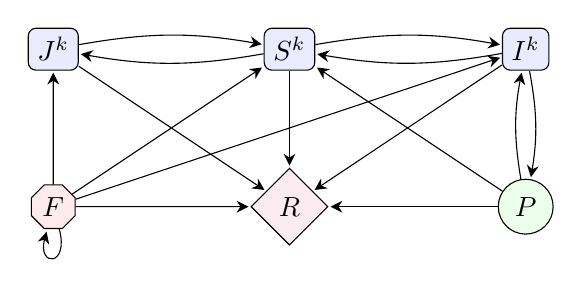
\begin{tikzpicture}[
  square/.style={rectangle, draw=black, minimum width=0.5cm, minimum height=0.5cm, rounded corners=.1cm, fill=blue!8},
  rhombus/.style={diamond, draw=black, minimum width=0.1cm, minimum height=0.1cm, fill=purple!8,aspect = 1},
  travel/.style={circle, draw=black, minimum width=0.5cm, minimum height=0.5cm, fill=green!8},
  report/.style={shape=regular polygon, regular polygon sides=8, draw, fill=red!8,minimum size=0.6cm,inner sep=0cm},
  bendy/.style={bend left=10},
  bendy2/.style={bend left=100},
  bendy3/.style={bend left=-100},
  >/.style={shorten >=0.25mm},
  >/.tip={Stealth[length=1.5mm,width=1.5mm]}
]
\tikzset{>={}};

\node (S) at (2.5,0) [square] {$S^{\species}$};
\node (I) at (5.5,0) [square] {$I^{\species}$};
\node (J) at (-0.5,0) [square] {$J^{\species}$};
\node (R) at (2.5,-2)  [rhombus] {$R$};
\node (P) at (5.5,-2)[travel] {$P$};
\node (F) at (-0.5,-2) [report] {$F$};



\draw [->, bendy] (S) to  (I);
\draw [->, bendy] (I) to  (S);
\draw [->, bendy] (J) to  (S);
\draw [->, bendy] (S) to  (J);


\draw [->] (P) --  (S);
\draw [->] (F) --  (R);
\draw [->] (P) --  (R);
\draw [->] (S) -- (R);
\draw [->] (I) -- (R);
\draw [->] (J) -- (R);
\draw [->] (F) -- (S);
\draw [->] (F) -- (J);
\draw [->] (F) -- (I);
\draw (F) edge[loop below] (F);

\draw [->, bendy] (P) to (I);
\draw [->, bendy] (I) to (P);


\end{tikzpicture}
}
\end{center}
\vspace{-5mm}
\caption{Flow diagram for the SIRJPF model illustrating population interactions. The model includes the $R$ state, representing mortality. Susceptible populations ($S^{\species}$) can reproduce into juvenile ($J^{\species}$), where the superscript $\species$ denotes the species of \textit{Daphnia}. And \textit{A.} Algae ($F$) will be refilled, as shown by the recycling arrows. Transitions from $S^{\species}$ to $I^{\species}$ denote infection, and transitions to the $R$ state occur upon death, where deceased individuals release parasites back into the environment. All $S^{\species}$, $I^{\species}$ and $J^{\species}$ consume resources from $F$, and over time, components in $F$ and $P$ also progress to $R$.}
\label{fig:flow_SIRJPF}
\end{figure}

\begin{figure}[H]
\centering
\begin{knitrout}
\definecolor{shadecolor}{rgb}{0.969, 0.969, 0.969}\color{fgcolor}
\includegraphics[width=\textwidth]{figure/DataVisSIRPFdent-1} 
\end{knitrout}
\caption{\label{fig:data_vis_SIRPF_dent}
Density (Individuals$/$Liter) of \textit{D.~dentifera}.
The top panel shows adult susceptibles (\textit{D.~dentifera}, black) and infecteds (\textit{D.~dentifera}, red).
The bottom panel shows juvenile susceptibles (\textit{D.~dentifera}, orange).
There were negligible infected juveniles.
Columns are buckets corresponding to replications with same treatment setting.
}
\end{figure}

\begin{figure}[H]
\centering
\begin{knitrout}
\definecolor{shadecolor}{rgb}{0.969, 0.969, 0.969}\color{fgcolor}
\includegraphics[width=\textwidth]{figure/DataVisSIRPFlum-1} 
\end{knitrout}
\caption{\label{fig:data_vis_SIRPF_lum}
Density (Individuals$/$Liter) of \textit{D.~lumholtzi}.
The top panel shows adult susceptibles (\textit{D.~lumholtzi}, blue) and infecteds (\textit{D.~lumholtzi}, green).
The bottom panel shows juvenile susceptibles (\textit{D.~lumholtzi}, purple).
There were negligible infected juveniles.
Columns are buckets corresponding to replications with same treatment setting.
}
\end{figure}

\subsection{Results}

\begin{table}[H]
\centering
\resizebox{\textwidth}{!}{
\begin{tabular}{||c|c |c|c|c||}
\hline
Parameter & Definition &Unit & Value & CI\\[0.5ex]
\hline
\hline
$S^{\native}$ & Susceptible host density   & $\mathrm{individual} \cdot L ^{-1}$                 & Variable                & \\
$I^{\native}$ & Infected host density     & $ \mathrm{individual} \cdot L ^{-1}$                & Variable                & \\
$J^{\native}$ & Juvenile host density    & $ \mathrm{individual} \cdot L ^{-1}$                & Variable                & \\
$F$   & Alga density                              & $10^6 \cdot \mathrm{cell} \cdot L ^{-1}$             & Variable                & \\
$P$   & Spore density                             & $10^3 \cdot \mathrm{spore} \cdot L ^{-1}$            & Variable                & \\
$r^{\native}$ &  Birth rate of juvenile                        & $\mathrm{individual} \cdot 10^{-6}\cdot \mathrm{cell}^{-1}$ & $5.52\cdot 10$  & ($3.67\cdot 10$,$1.68\cdot 10^{2}$)\\
$f^{\native}_{S}$ & Susceptible adult host filtering rate   &  $\mathrm{L} \cdot \mathrm{individual}^{-1} \cdot \mathrm{day}^{-1}$   & $7.64\cdot 10^{-4}$  & ($2.56\cdot 10^{-4}$,\,$1.31\cdot 10^{-3}$)\\
$p^{\native}$          & Number of infections per spore            &     $10^{-3} \cdot \mathrm{individual} \cdot \mathrm{spore}^{-1} $ & $3.06\cdot 10^{-1}$  & ($1.63\cdot 10^{-1}$,\,$8.67\cdot 10^{-1}$)\\
$p^{\native} \cdot f_{S^{\native}}$          & Effective infection rate of native adult hosts per‐spore      &     $10^{-3} \cdot \mathrm{L} \cdot \mathrm{spore}^{-1} \cdot \mathrm{day}^{-1}$  & $2.34\cdot 10^{-4}$  & ($1.77\cdot 10^{-4}$,$3.09\cdot 10^{-4}$)\\
$r^{\native} \cdot f_{S^{\native}}$          & Effective Birth rate of native juvenile            &     $10^{-6} \cdot \mathrm{L} \cdot \mathrm{cell}^{-1} \cdot \mathrm{day}^{-1} $ & $4.22\cdot 10^{-2}$  & ($3.81\cdot 10^{-2}$,$5.19\cdot 10^{-2}$)\\
$\theta^{\native}_{S}$ & Susceptible adult host mortality rate     &     $  \mathrm{day}^{-1}$     & $9.30\cdot 10^{-7}$  & (0,\,$1.83\cdot 10^{-4}$)\\
$\theta^{\native}_{I}$ & Infected adult host mortality rate        &     $  \mathrm{day}^{-1}$     & $4.54\cdot 10^{-1}$  & ($2.03\cdot 10^{-1}$,\,$7.57\cdot 10^{-1}$)\\
$\theta^{\native}_{J}$ & Juvenile mortality rate        &     $ \mathrm{day}^{-1}$     & $7.69\cdot 10^{-5}$  & (0,\,$4.43\cdot 10^{-2}$)\\
$\theta_{P}$   & Spore degradation rate                           &     $ \mathrm{day}^{-1}$     & $1.18\cdot 10^{-4}$   & (0,\,$2.15\cdot 10^{-2}$)\\
$\lambda^{\native}_{J}$ & Maturation rate of the juvenile                  &     $ \mathrm{day}^{-1} $                  & $1.00\cdot 10^{-1}$  & \\
$\xi$           & Ratio of infected host filtering rate       &     $\mathrm{Unitless}$                    & $1.13\cdot 10$         & ($2.48$,\,$4.37\cdot 10$)\\
$\xi_J$         & Ratio of juvenile individual filtering rate &     $\mathrm{Unitless}$                    & $1.00$ & \\
$\beta^{\native}$       & Spores produced by death per infected individual     &  $10^3 \cdot \mathrm{spore} \cdot \mathrm{individual}^{-1} \cdot \mathrm{day}^{-1}$  & $3.00\cdot 10$ & \\
$\mu$           & Algae refilling rate                                &  $10^6 \cdot \mathrm{cell} \cdot \mathrm{L} ^{-1} \cdot \mathrm{day}^{-1}$                 & $3.70\cdot 10^{-1}$ & \\
$\delta$        & Sampling rate                                      &  $day ^{-1}$                                                                         & $1.30\cdot 10^{-2}$ & \\
$\sigma^{\native}_{S}$ & Standard deviation of Brownian motion of susceptible adult         &   $\sqrt{\mathrm{individual} \cdot \mathrm{day}^{-1}}$  & 0  & \\
$\sigma^{\native}_{I}$ & Standard deviation of Brownian motion of infected adult         &   $\sqrt{\mathrm{individual} \cdot \mathrm{day}^{-1}}$  & $5.74\cdot 10^{-1}$  & (0,\,$6.19\cdot 10^{-1}$)\\
$\sigma^{\native}_{J}$ & Standard deviation of Brownian motion of juvenile               &   $\sqrt{\mathrm{individual} \cdot \mathrm{day}^{-1}}$  & $3.41\cdot 10^{-1}$  & ($1.52\cdot 10^{-1}$,\,$5.18\cdot 10^{-1}$)\\
$\sigma_{F}$   & Standard deviation of Brownian motion of alga                          &   $\sqrt{\mathrm{individual} \cdot \mathrm{day}^{-1}}$  & $6.97\cdot 10^{-2}$  & (0,\,$1.63\cdot 10^{-1}$)\\
$\sigma_{P}$   & Standard deviation of Brownian motion of parasite                      &   $\sqrt{\mathrm{individual} \cdot \mathrm{day}^{-1}}$  & $4.60\cdot 10^{-1}$  & ($2.10\cdot 10^{-1}$,\,$6.10\cdot 10^{-1}$)\\
$\tau^{\native}_{S}$      &  Measurement dispersion for susceptible adult                 &$\mathrm{Unitless}$           & $1.50\cdot 10$  & ($7.25$,\,$3.99\cdot 10$)\\
$\tau^{\native}_{I}$      &  Measurement dispersion for infected adult                &$\mathrm{Unitless}$            & $1.13$  & ($6.80\cdot 10^{-1}$,\,$2.61$)\\
\hline
\end{tabular}}
\caption{Variables and parameter definitions and estimates of SIRJPF model for \textit{D.~dentifera}-only dynamics. The confidence interval is generated by the Monte Carlo Adjusted Profile.}
\label{Table:SIRJPF_native}
\end{table}


\begin{table}[H]
\centering
\resizebox{\textwidth}{!}{
\begin{tabular}{||c|c |c|c|c||}
\hline
Parameter & Definition &Unit & Value & CI\\[0.5ex]
\hline
\hline
$S^{\invasive}$ & Susceptible host density   & $\mathrm{individual} \cdot L ^{-1}$                 & Variable                & \\
$I^{\invasive}$ & Infected host density     & $ \mathrm{individual} \cdot L ^{-1}$                & Variable                & \\
$J^{\invasive}$ & Juvenile host density    & $ \mathrm{individual} \cdot L ^{-1}$                & Variable                & \\
$F$   & Alga density                              & $10^6 \cdot \mathrm{cell} \cdot L ^{-1}$             & Variable                & \\
$P$   & Spore density                             & $10^3 \cdot \mathrm{spore} \cdot L ^{-1}$            & Variable                & \\
$r^{\invasive}$ &  Birth rate of juvenile                        & $\mathrm{individual} \cdot 10^{-6}\cdot \mathrm{cell}^{-1}$ & $2.49\cdot 10^{2}$  & ($9.36\cdot 10$,$1.63\cdot 10^{3}$)\\
$f^{\invasive}_{S}$ & Susceptible adult host filtering rate   &  $\mathrm{L} \cdot \mathrm{individual}^{-1} \cdot \mathrm{day}^{-1}$   & $6.49\cdot 10^{-4}$  & ($6.57\cdot 10^{-5}$,$1.33\cdot 10^{-3}$)\\
$p^{\invasive}$          & Number of infections per spore            &     $10^{-3} \cdot \mathrm{individual} \cdot \mathrm{spore}^{-1} $ & $6.65\cdot 10^{-1}$  & ($3.42\cdot 10^{-1}$,$6.17$)\\
$p^{\invasive} \cdot f_{S^{\invasive}}$          & Effective infection rate of invasive adult hosts per‐spore      &     $10^{-3} \cdot \mathrm{L} \cdot \mathrm{spore}^{-1} \cdot \mathrm{day}^{-1}$ & $4.32\cdot 10^{-4}$  & ($3.78\cdot 10^{-4}$,$7.45\cdot 10^{-4}$)\\
$r^{\invasive} \cdot f_{S^{\invasive}}$          & Effective Birth rate of invasive juvenile            &     $10^{-6} \cdot \mathrm{L} \cdot \mathrm{cell}^{-1} \cdot \mathrm{day}^{-1} $ & $1.62\cdot 10^{-1}$  & ($1.08\cdot 10^{-1}$,$2.48\cdot 10^{-1}$)\\
$\theta^{\invasive}_{S}$ & Susceptible adult host mortality rate     &     $ \mathrm{day}^{-1}$     & $5.73\cdot 10^{-1}$  & ($3.01\cdot 10^{-1}$,$1.16$)\\
$\theta^{\invasive}_{I}$ & Infected adult host mortality rate        &     $ \mathrm{day}^{-1}$     & $1.74\cdot 10^{-1}$  & ($2.05\cdot 10^{-2}$,$4.16\cdot 10^{-1}$)\\
$\theta^{\invasive}_{J}$ & Juvenile mortality rate        &     $  \mathrm{day}^{-1}$     & $2.55\cdot 10^{-5}$  & (0,$1.28\cdot 10^{-1}$)\\
$\theta_{P}$   & Spore degradation rate                           &     $ \mathrm{day}^{-1}$     & $1.71\cdot 10^{-6}$   & (0,$8.61\cdot 10^{-2}$)\\
$\lambda^{\invasive}_{J}$ & Maturation rate of the juvenile                  &     $ \mathrm{day}^{-1} $                  & $1.00\cdot 10^{-1}$  & \\
$\xi$           & Ratio of infected host filtering rate       &     $\mathrm{Unitless}$                    & $7.33\cdot 10$         & ($9.54$,$8.02\cdot 10^{2}$)\\
$\xi_J$         & Ratio of juvenile individual filtering rate &     $\mathrm{Unitless}$                    & $1.00$ & \\
$\beta^{\invasive}$       & Spores produced by death per infected individual     &  $10^3 \cdot \mathrm{spore} \cdot \mathrm{individual}^{-1} \cdot \mathrm{day}^{-1}$  & $3.00\cdot 10$ & \\
$\mu$           & Algae refilling rate                                &  $10^6 \cdot \mathrm{cell} \cdot \mathrm{L} ^{-1} \cdot \mathrm{day}^{-1}$                 & $3.70\cdot 10^{-1}$ & \\
$\delta$        & Sampling rate                                      &  $day ^{-1}$                                                                         & $1.30\cdot 10^{-2}$ & \\
$\sigma^{\invasive}_{S}$ & Standard deviation of Brownian motion of susceptible adult         &   $\sqrt{\mathrm{individual} \cdot \mathrm{day}^{-1}}$  & 0  & \\
$\sigma^{\invasive}_{I}$ & Standard deviation of Brownian motion of infected adult         &   $\sqrt{\mathrm{individual} \cdot \mathrm{day}^{-1}}$  & $2.73\cdot 10^{-1}$  & (0, $5.75\cdot 10^{-1}$)\\
$\sigma^{\invasive}_{J}$ & Standard deviation of Brownian motion of juvenile               &   $\sqrt{\mathrm{individual} \cdot \mathrm{day}^{-1}}$  & $3.72\cdot 10^{-1}$  & ($2.75\cdot 10^{-1}$, $5.25\cdot 10^{-1}$)\\
$\sigma_{F}$   & Standard deviation of Brownian motion of alga                          &   $\sqrt{\mathrm{individual} \cdot \mathrm{day}^{-1}}$  & $5.22\cdot 10^{-8}$  & (0,$1.80\cdot 10^{-2}$)\\
$\sigma_{P}$   & Standard deviation of Brownian motion of parasite                      &   $\sqrt{\mathrm{individual} \cdot \mathrm{day}^{-1}}$  & $7.99\cdot 10^{-8}$  & (0,$3.55\cdot 10^{-1}$)\\
$\tau^{\invasive}_{S}$      &  Measurement dispersion for susceptible adult                  &$\mathrm{Unitless}$           & $7.00\cdot 10$  & (0,$4.40\cdot 10^{3}$)\\
$\tau^{\invasive}_{I}$      &  Measurement dispersion for infected adult                 &$\mathrm{Unitless}$            & $1.17$  & ($5.80\cdot 10^{-1}$,$1.08\cdot 10$)\\
\hline
\end{tabular}}
\caption{Variables and parameter definitions and estimates of SIRJPF model for \textit{D.~lumholtzi}-only dynamics. The confidence interval is generated by the Monte Carlo Adjusted Profile.}
\label{Table:SIRJPF_invasive}
\end{table}

\begin{figure}[H]
    \centering
    \includegraphics[width=\linewidth]{profile/Simple_dynamics/Dent/para/Profile_plot.png}
    \caption{Monte Carlo Adjusted Profile results of SIRJPF model for \textit{D.~dentifera}-only dynamics.
    The vertical dotted lines represent the 95\% confidence interval obtained by MCAP.
    The vertical blue lines show the MLE estimated using MCAP.
    The red vertical lines correspond to the model with the overall highest likelihood among all searches.
    }
    \label{fig:SIRJPF_dent_profile}
\end{figure}

\begin{figure}[H]
    \centering
    \includegraphics[width=\linewidth]{profile/Simple_dynamics/Lum/para/Profile_plot.png}
    \caption{Monte Carlo Adjusted Profile results of SIRJPF model for \textit{D.~lumholtzi}-only dynamics.
    The vertical dotted lines represent the 95\% confidence interval obtained by MCAP.
    The vertical blue lines show the MLE estimated using MCAP.
    The red vertical lines correspond to the model with the overall highest likelihood among all searches.
}
    \label{fig:SIRJPF_native_profile}
\end{figure}

\begin{table}[h!]
\centering
\begin{center}
\begin{tabular}{||c |c |c |c|c|c||}
 \hline
Specific parameters  & Max log-likelihood & AIC & \makecell[c]{Max log-likelihood\\(block)} & \makecell[c]{AIC\\(block)} & \makecell[c]{LRT\\$p$-value}\\ [0.5ex]
 \hline\hline
$\theta^{\native}_{I,\unit}$ & -549.38& 1140.77& -547.92& 1137.84 & $<$0.001 \\
$\varnothing$  & -567.98& 1163.97& -567.98& 1163.97 & --- \\
 $r^{\native}_{\unit}$ & -563.38& 1168.76& -562.95& 1167.90 & 0.24 \\
$p^{\native}_{\unit}$ & -563.78& 1169.56& -562.75& 1167.49 & 0.30 \\
$\xi_{\unit}$ & -566.59& 1175.19& -565.80& 1173.60 & 0.90 \\
$\theta^{\native}_{S,\unit}$ & -567.31& 1176.61& -565.48& 1172.96 & 0.99 \\
$f^{\native}_{S,\unit}$ & -568.66& 1179.33& -566.32& 1174.63 & $>$0.99 \\
$\theta_{P,\unit}$& -568.21& 1178.42& -568.87& 1179.74 & $>$0.99 \\[1ex]
 \hline
\end{tabular}
\end{center}
\caption{Comparison of model fit and complexity across various configurations of unit-specific parameters within the panelPOMP framework for \textit{D.~dentifera}-only dynamics. The unit-specific parameter setting assessed include $\theta^{\native}_{I,\unit}$, $p^{\native}_{\unit}$, $r^{\native}_{\unit}$, $\xi_{\unit}$, $\theta^{\native}_{S,\unit}$, $\theta_{P,\unit}$.}
\label{Table:SIRJPF_dent_model_comparison}
\end{table}

\begin{table}[h!]
\centering
\begin{center}
\begin{tabular}{||c |c |c |c|c|c||}
 \hline
Specific parameters  & Max log-likelihood & AIC & \makecell[c]{Max log-likelihood\\(block)} & \makecell[c]{AIC\\(block)} & \makecell[c]{LRT\\$p$-value}\\ [0.5ex]
 \hline\hline
$\xi_{\unit}$ & -419.78& 883.560& -416.87& 877.747 & 0.03 \\
$\varnothing$  & -428.36& 884.715& -428.36& 884.715 & --- \\
$p^{\invasive}_{\unit}$ & -421.21& 886.411& -420.66& 885.326 & 0.07 \\
$\theta^{\invasive}_{I,\unit}$ & -421.21& 886.427& -419.32& 882.636 & 0.07 \\
$f^{\invasive}_{S,\unit}$ & -422.85& 889.700& -423.26& 890.523 & 0.20 \\
$\theta_{P,\unit}$ & -429.20& 902.400& -428.99& 901.972 & $>$0.99 \\
$r^{\invasive}_{\unit}$ & -432.43& 908.868& -426.31& 896.612 & $>$0.99 \\
$\theta^{\invasive}_{S,\unit}$ & -432.87& 909.740& -430.01& 904.014 & $>$0.99 \\[1ex]
 \hline
\end{tabular}
\end{center}
\caption{Comparison of model fit and complexity across various configurations of unit-specific parameters within the panelPOMP framework for \textit{D.~lumholtzi}-only dynamics. The unit-specific parameter setting assessed include $\theta^{\invasive}_{I,\unit}$, $p^{\invasive}_{\unit}$, $r^{\invasive}_{\unit}$, $\xi_{\unit}$, $\theta^{\invasive}_{S,\unit}$, $\theta_{P,\unit}$.}
\label{Table:SIRJPF_lum_model_comparison}
\end{table}

Despite the model configuration with unit-specific $\theta^{\native}_{I,\unit}$ and $\xi_{\unit}$ achieving the lowest AIC value in Table \ref{Table:SIRJPF_dent_model_comparison} and \ref{Table:SIRJPF_lum_model_comparison}, the improvement over the all-shared-parameters model is marginal.
This slight advantage may be attributed to Monte Carlo error inherent in the parameter estimation process using the panelPOMP framework.
The stochastic nature of the iterated filtering algorithms employed in POMP relies on Monte Carlo simulations, which can introduce variability in the maximum likelihood estimates and, consequently, the AIC values.
The LRT $p$-values in Tables~\ref{Table:SIRJPF_dent_model_comparison} and~\ref{Table:SIRJPF_lum_model_comparison} further support this conclusion: none of the unit-specific models achieve a statistically significant improvement over the all-shared model, consistent with the AIC-based ranking.
\parskip 3mm

Given the potential for such computational noise, the relatively small difference in AIC, and the lack of significant LRT $p$-values, we prefer to adopt the model with all shared parameters.
This choice promotes parsimony and reduces the risk of overfitting, ensuring that the model remains both interpretable and generalizable.
By keeping $\theta_I$—the natural death rate of infected \textit{Daphnia}—shared across all units, we maintain a simpler model structure that is sufficient to describe the observed data without unnecessary complexity.

\subsection{Simulation}
The simulation plots (Figures \ref{fig:SIRJPF_native_simulation_band} to \ref{fig:SIRJPF_lum_simulation_lines}) demonstrate our model's capability to capture the complex interactions among various states within the population dynamics of \textit{D.~dentifera} and \textit{D.~lumholtzi}.
Specifically, the model captures the latent pattern for susceptible and infected densities across multiple experimental units, as evidenced by the close alignment between the simulated mean trajectories (depicted by the black and light-blue bands) and the observed experimental data (colorful solid lines).
Each blue line represents an individual simulation case, capturing the stochastic variability across replicates, while the light blue shaded area (where present) denotes the 95\% confidence interval of the simulation results.
Remarkably, although juvenile density data were not included in the model fitting process, the model still effectively predicts juvenile density trends.
The promising performance of the model indicates the model's capacity to generalize underlying ecological processes, as the 95\% confidence intervals largely cover the observed juvenile data.

\parskip 3mm

At the same time, the depletion of  algal density over time, reflected in the simulation further explains the behavior of the \textit{Daphnia}.
The decline in algal density at later stages indicates that the system reaches a state of food limitation, which is a dynamic anticipated by our model.
The reduction in food availability provides a mechanistic explanation for the observed trends in \textit{Daphnia} densities, as resource scarcity constrains population growth, ultimately affecting the susceptible, infected, and juvenile densities.
Thus, the model captures not only the reproductive dynamics but also the resource-consumption interactions that shape these dynamics.
The model’s ability to reproduce these patterns accurately highlights its potential utility in explaining and predicting empirical trends in complex ecological systems.



\begin{figure}[H]
    \centering
    \includegraphics[width=0.75\linewidth]{simulation/dent_para_simulation/simulation_band.png}
    \caption{Simulation plots of densities (Individuals$/$Liter) for susceptible, infected, and juvenile \textit{D.~dentifera}, along with alga density ($10^6\cdot$cells$/$Liter) and parasite density ($10^3\cdot$spores$/$Liter), over time (days). The colorful solid lines represent observed experimental data, showing the variability across different experimental replicates. The black line represents the mean trajectory from the simulation model, capturing the general trend of each density. The light blue shaded area corresponds to the 95\% confidence interval of the simulations, indicating the range of model predictions. Dashed lines illustrate individual simulated trajectories, highlighting the model’s ability to capture fluctuations around the mean trajectory.}
    \label{fig:SIRJPF_native_simulation_band}
\end{figure}


\begin{figure}[H]
    \centering
    \includegraphics[width=0.75\linewidth]{simulation/dent_para_simulation/simulation_lines.png}
   \caption{Simulated densities (Individuals$/$Liter) of susceptible \textit{D.~dentifera}, infected \textit{D.~dentifera} density, juvenile \textit{D.~dentifera} and alga density ($10^6\cdot$cells$/$Liter) over time (days) for each experimental unit. The blue lines represent individual simulation runs, capturing the variability in susceptible density across replicates, while the red line represents the actual experimental data.}
    \label{fig:SIRJPF_dent_simulation_lines}
\end{figure}



\begin{figure}[H]
    \centering
    \includegraphics[width=0.75\linewidth]{simulation/lum_para_simulation/simulation_band.png}
    \caption{Simulation plots of densities (Individuals$/$Liter) for susceptible, infected, and juvenile \textit{D.~lumholtzi}, along with alga density ($10^6\cdot$cells$/$Liter) and parasite density ($10^3\cdot$spores$/$Liter), over time (days). The colorful solid lines represent observed experimental data, showing the variability across different experimental replicates. The black line represents the mean trajectory from the simulation model, capturing the general trend of each density. The light blue shaded area corresponds to the 95\% confidence interval of the simulations, indicating the range of model predictions. Dashed lines illustrate individual simulated trajectories, highlighting the model’s ability to capture fluctuations around the mean trajectory.}
    \label{fig:SIRJPF_invasive_simulation_band}
\end{figure}

\begin{figure}[H]
    \centering
    \includegraphics[width=0.75\linewidth]{simulation/lum_para_simulation/simulation_lines.png}
   \caption{Simulated trajectories of susceptible \textit{D.~lumholtzi}, infected \textit{D.~lumholtzi}, juvenile \textit{D.~lumholtzi} and alga density ($10^6\cdot$cells$/$Liter) over time (days) for each experimental unit (u1 to u9). The blue lines represent individual simulation runs, capturing the variability in susceptible density across replicates, while the red line represents the actual experimental data.}
    \label{fig:SIRJPF_lum_simulation_lines}
\end{figure}


\section{SRJF2 Model}
In this section, we introduce the SRJF2 model, which analyze the dynamics between native and invasive species competing for a shared food resource, algae ($F$) in each bucket($\unit$).
The stochastic differential equations governing the system are:
{\small
\begin{align}
    dS^{\species}_{\unit}(t) &= \lambda^{\species}_{J,{\unit}} J^{\species}_{\unit}(t) \, dt - (\theta^{\species}_{S,{\unit}} + \delta) S^{\species}_{\unit}(t)\, dt + S^{\species}_{\unit}(t)\, d\zeta^{\species}_{S,{\unit}}, \label{eq:SRJF2_dS}\\
    dJ^{\species}_{\unit}(t) &= r^{\species}_{\unit}f^{\species}_{S,{\unit}}F_{\unit}(t) S^{\species}_{\unit}(t)\, dt - \theta^{\species}_{J,{\unit}} J^{\species}_{\unit}(t)\, dt - \delta J^{\species}_{\unit}(t)\, dt - \lambda^{\species}_{J,{\unit}} J^{\species}_{\unit}(t)\, dt + J^{\species}_{\unit}(t)\, d\zeta^{\species}_{J,{\unit}}, \label{eq:SRJF2_dJ}\\
    dF_{\unit}(t) &= - \sum_{\species \in \{\native, \invasive\}} f^{\species}_{S,{\unit}} F_{\unit}(t) \left(S^{\species}_{\unit}(t)+\xi_{J,{\unit}}J^{\species}_{\unit}(t)\right)dt  + \mu \, dt + F_{\unit}(t)\, d\zeta_{F,{\unit}}, \label{eq:SRJF2_dF}\\
d\zeta^{\species}_{S,{\unit}} &\sim \Normal \big[0, (\sigma^{\species}_{S,{\unit}})^{2}\, dt\big]\,
d\zeta^{\species}_{J,{\unit}} \sim \Normal \big[0, (\sigma^{\species}_{J,{\unit}})^{2}\, dt\big]\,
d\zeta_{F,{\unit}} \sim \Normal \big[0, \sigma_{F,{\unit}}^{2}\, dt\big]\label{eq:SRJF2_dzetaS}.
\end{align}
}
Equation~\eqref{eq:SRJF2_dS} models the rate of change of the specific species' susceptible population $S^{\species}_{\unit}(t)$.
The term $\lambda^{\species}_{J,\unit} J^{\species}_{\unit}(t) \, dt$ represents the maturation of juveniles into susceptible adults at rate $\lambda^{\species}_{J,\unit}$.
The mortality term $-\left(\theta^{\species}_{S,\unit} + \delta\right) S^{\species}_{\unit}(t) \, dt$ accounts for natural death at rate $\theta^{\species}_{S,\unit}$ and the sampling rate $\delta$.
For consistency with the SIRJPF2 and SIRJPF model, we further fix $\sigma^{\species}_{S,{\unit}}$ to be zero for specific analysis of this dynamics.
\parskip 3mm

Equation~\eqref{eq:SRJF2_dJ} describes the dynamics of the juvenile population $J^{\species}_{\unit}(t)$.
The growth term $r^{\species}_{\unit} f^{\species}_{S,\unit} F_{\unit}(t) S^{\species}_{\unit}(t) \, dt$ signifies the production of juveniles through reproduction, where $r^{\species}_{\unit}$ is the growth factor and $f^{\species}_{S,\unit}$ is the filtering rate of susceptible individuals on algae.
The loss term $-\left(\theta^{\species}_{J,\unit} + \delta + \lambda^{\species}_{J,\unit}\right) J^{\species}(t) \, dt$ includes natural juvenile mortality at rate $\theta^{\species}_{J,\unit}$, sampling rate $\delta$, and maturation into the susceptible adult class at rate $\lambda^{\species}_{J,\unit}$.
The stochastic term $J^{\species}_{\unit}(t) \, d\zeta^{\species}_{J,\unit}$ captures random fluctuations affecting the juvenile population, with $d\zeta^{\species}_{J,\unit}$ being the Brownian motion characterized by variance $(\sigma^{\species}_{J,{\unit}})^{2}\, dt$.
\parskip 3mm

Equation~\eqref{eq:SRJF2_dF} captures the dynamics of the algae population $F_{\unit}(t)$, which serves as a shared food resource for both native and invasive species.
The consumption terms $\sum_{\species \in \{\native, \invasive\}} f^{\species}_{S,{\unit}} F_{\unit}(t) \left(S^{\species}_{\unit}(t)+\xi_{J,{\unit}}J^{\species}_{\unit}(t)\right)dt$ represent the reduction of algae due to feeding by native and invasive susceptible individuals and juveniles, respectively.
The parameter $\xi_{J,\unit}$ denotes the relative ratio of juveniles on algae consumption compared to susceptible adults.
The term $\mu \, dt$ represents the refill rate of algae, contributing to its replenishment.
The stochastic fluctuation $F_{\unit}(t) \, d\zeta_{F,\unit}$ introduces randomness into the algae dynamics, where $d\zeta_{F,\unit}$ is the Brownian motion with variance $\sigma_{F,{\unit}}^{2}\, dt$.
\parskip 3mm

The following Figure~\ref{fig:SRJF2} presents the flow diagram of the SRJF2 model, illustrating the interactions among susceptible individuals ($S^{\native}$, $S^{\invasive}$), juveniles ($J^{\native}$,$J^{\invasive}$), algae as a food resource ($F$), and mortality ($R$).
The bidirectional arrows between $J^{\species}$ and $S^{\species}$, represent the maturation of juveniles into susceptible individuals and the reproduction of susceptible individuals into juveniles.
Both susceptible individuals and juveniles, consume resources from the alga population $F$, as indicated by the arrows from $F$ to each population node.
The algal food resource is regularly replenished, depicted by the recycling loop, and contributes to the growth of both susceptible individuals and juveniles.
All populations have pathways leading to the mortality state $R$, representing natural death and disease-induced mortality.
Two species of \textit{Daphnia} are competing through the food resources in this model.

\begin{figure}[H]
\begin{center}
%%%%% SRJF2 diagram
\resizebox{8cm}{!}{
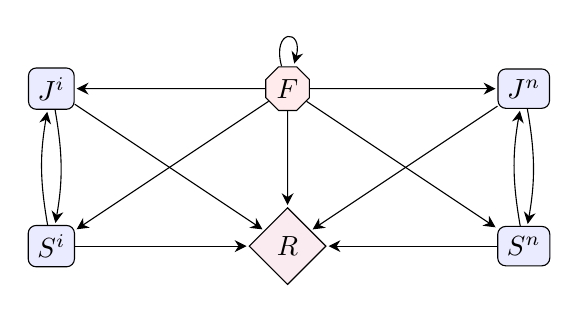
\begin{tikzpicture}[
  square/.style={rectangle, draw=black, minimum width=0.5cm, minimum height=0.5cm, rounded corners=.1cm, fill=blue!8},
  rhombus/.style={diamond, draw=black, minimum width=0.1cm, minimum height=0.1cm, fill=purple!8,aspect = 1},
  travel/.style={circle, draw=black, minimum width=0.5cm, minimum height=0.5cm, fill=green!8},
  report/.style={shape=regular polygon, regular polygon sides=8, draw, fill=red!8,minimum size=0.6cm,inner sep=0cm},
  bendy/.style={bend left=10},
  bendy2/.style={bend left=100},
  bendy3/.style={bend left=-100},
  >/.style={shorten >=0.25mm},
  >/.tip={Stealth[length=1.5mm,width=1.5mm]}
]
\tikzset{>={}};

\node (Sn) at (5.5,0) [square] {$S^{\native}$};
\node (Si) at (-0.5,0) [square] {$S^{\invasive}$};
\node (Jn) at (5.5,2) [square] {$J^{\native}$};
\node (Ji) at (-0.5,2) [square] {$J^{\invasive}$};
\node (R) at (2.5,0)  [rhombus] {$R$};
\node (F) at (2.5,2) [report] {$F$};



\draw [->, bendy] (Jn) to  (Sn);
\draw [->, bendy] (Ji) to  (Si);
\draw [->, bendy] (Sn) to  (Jn);
\draw [->, bendy] (Si) to  (Ji);


\draw [->] (F) --  (R);
\draw [->] (Sn) -- (R);
\draw [->] (Si) -- (R);
\draw [->] (Jn) -- (R);
\draw [->] (Ji) -- (R);
\draw [->] (F) -- (Sn);
\draw [->] (F) -- (Si);
\draw [->] (F) -- (Jn);
\draw [->] (F) -- (Ji);
\draw (F) edge[loop above] (F);


\end{tikzpicture}
}
\end{center}
\vspace{-5mm}
\caption{Flow diagram for the SRJF2 model illustrating population interactions. The model includes the $R$ state, representing mortality. For $\species \in \{\native,\invasive\}$, Susceptible populations ($S^{\species}$) can reproduce into juvenile ($J^{\species}$). And \textit{A.} Algae ($F$) will be refilled, as shown by the recycling arrows. Both $S^{\species}$ and $J^{\species}$ consume resources from $F$, and over time, components in $F$ also progress to $R$.}
\label{fig:SRJF2}
\end{figure}

\begin{figure}[H]
\centering
\begin{knitrout}
\definecolor{shadecolor}{rgb}{0.969, 0.969, 0.969}\color{fgcolor}
\includegraphics[width=\textwidth]{figure/DataVisSRJF2-1} 
\end{knitrout}
\caption{\label{fig:data_vis_SRJF2}
Density (Individuals$/$Liter) of \textit{D.~dentifera} (solid lines) and \textit{D.~lumholtzi} (dashed lines).
The top panel shows adult susceptibles (\textit{D.~dentifera}, black and \textit{D.~lumholtzi}, blue).
The bottom panel shows juvenile susceptibles (\textit{D.~dentifera}, orange; \textit{D.~lumholtzi}, purple).
There were negligible infected juveniles.
Columns are buckets corresponding to replications with same treatment setting.
}
\end{figure}

\subsection{Results}

\begin{table}[H]
\centering
\resizebox{\textwidth}{!}{
\begin{tabular}{||c|c |c|c|c||}
\hline
Parameter & Definition &Unit & Value & CI\\[0.5ex]
\hline
\hline
$S^{\species}$ & Susceptible host density for species $\species$  & $\mathrm{individual} \cdot L ^{-1}$                 & Variable                & \\
$J^{\species}$ & Juvenile host density for species $\species$     & $ \mathrm{individual} \cdot L ^{-1}$                & Variable                & \\
$F$   & Alga density                              & $10^6 \cdot \mathrm{cell} \cdot L ^{-1}$             & Variable                & \\
$P$   & Spore density                             & $10^3 \cdot \mathrm{spore} \cdot L ^{-1}$            & Variable                & \\
$r^{\native}$ & Birth rate of native juvenile                        & $\mathrm{individual} \cdot 10^{-6}\cdot \mathrm{cell}^{-1}$ & $6.29\cdot 10^{3}$  & ($2.42\cdot 10^{3}$,$3.76\cdot 10^{4}$)\\
$r^{\invasive}$ & Birth rate of invasive juvenile                      & $\mathrm{individual} \cdot 10^{-6}\cdot \mathrm{cell}^{-1}$ & $4.75\cdot 10^{3}$  & ($1.78\cdot 10^{3}$,$6.79\cdot 10^{4}$)\\
$f^{\native}_{S}$ & Native susceptible adult host filtering rate   &  $\mathrm{L} \cdot \mathrm{individual}^{-1} \cdot \mathrm{day}^{-1}$   & $7.10\cdot 10^{-5}$  & ($1.54\cdot 10^{-5}$,$1.17\cdot 10^{-4}$)\\
$f^{\invasive}_{S}$ & Invasive susceptible adult host filtering rate &  $\mathrm{L} \cdot \mathrm{individual}^{-1} \cdot \mathrm{day}^{-1}$   & $8.90\cdot 10^{-5}$  & (0,$2.04\cdot 10^{-4}$)\\
$r^{\native} \cdot f_{S^{\native}}$          & Effective Birth rate of native juvenile            &     $10^{-6} \cdot \mathrm{L} \cdot \mathrm{cell}^{-1} \cdot \mathrm{day}^{-1} $ & $4.47\cdot 10^{-1}$  & ($3.18\cdot 10^{-1}$,$1.16$)\\
$r^{\invasive} \cdot f_{S^{\invasive}}$          & Effective Birth rate of invasive juvenile            &     $10^{-6} \cdot \mathrm{L} \cdot \mathrm{cell}^{-1} \cdot \mathrm{day}^{-1} $ & $4.23\cdot 10^{-1}$  & ($2.67\cdot 10^{-1}$,$3.55$)\\
$\theta^{\native}_{S}$ & Native susceptible adult host mortality rate     &     $  \mathrm{day}^{-1}$     & $1.03$  & ($4.63\cdot 10^{-1}$,$1.86$)\\
$\theta^{\invasive}_{S}$ & Invasive susceptible adult host mortality rate   &     $  \mathrm{day}^{-1}$     & $4.49\cdot 10^{-1}$  & ($3.12\cdot 10^{-1}$,$1.40$)\\
$\theta^{\native}_{J}$ & Native juvenile mortality rate        &     $   \mathrm{day}^{-1}$     & $2.13\cdot 10^{-1}$  & ($7.94\cdot 10^{-2}$,$9.35\cdot 10^{-1}$)\\
$\theta^{\invasive}_{J}$ & Invasive juvenile mortality rate      &     $  \mathrm{day}^{-1}$     & $7.35\cdot 10^{-1}$  & ($2.91\cdot 10^{-1}$,$4.08$)\\
$\lambda^{\native}_{J}$ & Maturation rate of native juvenile                  &     $ \mathrm{day}^{-1} $                  & $1.00\cdot 10^{-1}$  & \\
$\lambda^{\invasive}_{J}$ & Maturation rate of invasive juvenile                &     $ \mathrm{day}^{-1} $                  & $1.00\cdot 10^{-1}$  & \\
$\xi_J$         & Ratio of juvenile individual filtering rate &     $\mathrm{Unitless}$                    & $1.00$ & \\
$\beta^{\native}$       & Spores produced per infected native individual     &  $10^3 \cdot \mathrm{spore} \cdot \mathrm{individual}^{-1} \cdot \mathrm{day}^{-1}$  & $3.00\cdot 10$ & \\
$\beta^{\invasive}$       & Spores produced per infected invasive individual   &  $10^3 \cdot \mathrm{spore} \cdot \mathrm{individual}^{-1} \cdot \mathrm{day}^{-1}$  & $3.00\cdot 10$ & \\
$\mu$           & Alga refilling rate                                &  $10^6 \cdot \mathrm{cell} \cdot \mathrm{L} ^{-1} \cdot \mathrm{day}^{-1}$                 & $3.70\cdot 10^{-1}$ & \\
$\delta$        & Sampling rate                                      &  $day ^{-1}$                                                                         & $1.30\cdot 10^{-2}$ & \\
$\sigma^{\native}_{S}$ & Standard deviation of Brownian motion of native susceptible adult             &   $\sqrt{\mathrm{individual} \cdot \mathrm{day}^{-1}}$  & 0  & \\
$\sigma^{\invasive}_{S}$ & Standard deviation of Brownian motion of invasive susceptible adult              &   $\sqrt{\mathrm{individual} \cdot \mathrm{day}^{-1}}$  & 0  & \\
$\sigma^{\native}_{J}$ & Standard deviation of Brownian motion of native juvenile               &   $\sqrt{\mathrm{individual} \cdot \mathrm{day}^{-1}}$  & $2.79\cdot 10^{-1}$  & ($1.38\cdot 10^{-1}$,$4.45\cdot 10^{-1}$)\\
$\sigma^{\invasive}_{J}$ & Standard deviation of Brownian motion of invasive juvenile             &   $\sqrt{\mathrm{individual} \cdot \mathrm{day}^{-1}}$  & $4.99\cdot 10^{-4}$  & ($5.87\cdot 10^{-5}$,$7.10\cdot 10^{-2}$)\\
$\sigma_{F}$   & Standard deviation of Brownian motion of alga                          &   $\sqrt{\mathrm{individual} \cdot \mathrm{day}^{-1}}$  & $5.37\cdot 10^{-2}$  & ($2.72\cdot 10^{-2}$,$9.19\cdot 10^{-2}$)\\
$\tau^{\native}_{S}$      &  Measurement dispersion for susceptible native adult             &$\mathrm{Unitless}$           & $1.12\cdot 10$  & ($4.26$,$1.10\cdot 10^{2}$)\\
$\tau^{\invasive}_{S}$      &  Measurement dispersion for susceptible invasive adult              &$\mathrm{Unitless}$            & $2.43$  & ($1.55$,$4.44$)\\
\hline
\end{tabular}}
\caption{Variables and parameter definitions and estimates of SRJF2 model for dynamics with both species of \textit{Daphnia}. The confidence interval is generated by the Monte Carlo Adjusted Profile.}
\label{Table:SRJF2}
\end{table}

\begin{figure}[H]
    \centering
    \includegraphics[width=\linewidth]{profile/Target_dynamics/no_para/Profile_plot.png}
    \caption{Monte Carlo Adjusted Profile results of SRJF2 model for dynamics with both species of \textit{Daphnia}.
    The vertical dotted lines represent the 95\% confidence interval obtained by MCAP.
    The vertical blue lines show the MLE estimated using MCAP.
    The red vertical lines correspond to the model with the overall highest likelihood among all searches.
}
    \label{fig:SRJF2_profile}
\end{figure}


\begin{table}[h!]
\centering
\begin{center}
\begin{tabular}{||c |c |c |c|c|c||}
 \hline
Specific parameters  & Max log-likelihood & AIC & \makecell[c]{Max log-likelihood\\(block)} & \makecell[c]{AIC\\(block)} & \makecell[c]{LRT\\$p$-value}\\ [0.5ex]
 \hline\hline
$\varnothing$  & -701.17& 1428.34& -701.17& 1428.34 & --- \\
$\theta^{\species}_{S,\unit}$ & -705.50& 1468.99& -691.20& 1440.39 & $>$0.99 \\
$f^{\species}_{S,\unit}$ & -720.72& 1499.44& -692.71& 1443.43 & $>$0.99 \\
$r^{\species}_{\unit}$  & -725.74& 1509.49& -696.35& 1450.70 & $>$0.99 \\[1ex]
 \hline
\end{tabular}
\end{center}
\caption{Comparison of model fit and complexity across various configurations of unit-specific parameters within the panelPOMP framework with SRJF2 model for dynamics with both species of \textit{Daphnia}. The unit-specific parameter setting assessed include (1)$\theta^{\species}_{S,\unit}$, (2)$f^{\species}_{S,\unit}$ , and (3)$r^{\species}_{\unit}$ for $\species \in \{\native,\invasive\}$.}
\label{Table:SRJF2_model_comparison}
\end{table}

Table~\ref{Table:SRJF2_model_comparison} presents a comparison of model fit and complexity across various configurations of unit-specific parameters within the panelPOMP framework for the SRJF2 model, which captures the dynamics of both native and invasive \textit{Daphnia} species.
We employed MCAP methods to estimate the maximum log-likelihood and AIC for each model configuration.
The models assessed include those with unit-specific parameters for the mortality rates ($\theta^{\species}_{S,\unit}$), filter rates ($f^{\species}_{S,\unit}$), and growth efficiency factors ($r^{\species}_{\unit}$) for $\species \in \{\native,\invasive\}$.
The model with all parameters shared (no unit-specific parameters) achieves the minimum AIC, indicating the best balance between model fit and complexity.
The LRT $p$-values confirm that none of the unit-specific parameterizations provide a statistically significant improvement over the all-shared baseline, corroborating the AIC-based selection.
Consequently, we choose to retain the model with all shared parameters, as it offers a more parsimonious representation of the system dynamics without compromising the explanatory power.

\subsection{Simulation}
The simulation results presented in Figures \ref{fig:SRJF2_simulation_band} to \ref{fig:SRJF2_simulation_lines} showcase our model's ability to represent the complex population interactions between \textit{D.~dentifera} and \textit{D.~lumholtzi}.
The model captures the patterns of susceptible and juvenile densities across multiple experimental units, as evidenced by the close alignment of the simulated mean trajectories (illustrated by the black line and light blue confidence bands) with the experimental data (shown by the colorful solid lines).
Despite the fact that juvenile density data were not used in calibrating the model, the model accurately predicts juvenile density trends, indicating its capability to generalize ecological processes effectively.
The 95\% confidence intervals largely encompass the observed juvenile data, supporting the construction of the model's latent process.

\parskip 3mm

Figure \ref{fig:SRJF2_simulation_lines} provides further insight into the dynamics of algal depletion over time, an aspect that is integral to the model’s predictions for \textit{Daphnia} populations.
The observed decrease in algal density at later stages, captured in the simulations, suggests a shift to a resource-limited environment—a behavior that aligns well with our model's assumptions.
As algae availability declines, population growth of both susceptible and juvenile \textit{Daphnia} becomes constrained, providing a mechanistic explanation for the observed patterns in their densities.
By incorporating resource-consumption feedback into the population dynamics, the model demonstrates not only an ability to simulate individual population trends but also to capture this ecological feedback loop.


\begin{figure}
    \centering
    \includegraphics[width=0.75\linewidth]{simulation/target_no_para_simulation/simulation_band.png}
    \caption{Simulation plots of densities (Individuals$/$Liter) for susceptible and juvenile populations of both native \textit{D.~dentifera} and invasive \textit{D.~lumholtzi}, along with alga density ($10^6\,$cells$/$Liter) over time (days). Colorful solid lines represent observed experimental data for each experimental replicate, showcasing variability across replicates. The black line represents the mean simulation trajectory, while the light blue shaded area corresponds to the 95\% confidence interval of the simulation. Dashed lines indicate individual simulation cases, illustrating the model's capacity to capture fluctuations around the mean trajectory.}
    \label{fig:SRJF2_simulation_band}
\end{figure}

\begin{figure}
    \centering
    \includegraphics[width=0.75\linewidth]{simulation/target_no_para_simulation/simulation_lines.png}
    \caption{Simulated density ($10^6\,$cells$/$Liter) of susceptible native \textit{D.~dentifera}, susceptible invasive \textit{D.~lumholtzi}, juvenile native \textit{D.~dentifera}, invasive \textit{D.~lumholtzi}, and alga density ($F$) over time (days) for each experimental unit. The blue lines represent individual simulation cases, while the red line denotes observed experimental data, showing how simulated variability compares to actual data.}
    \label{fig:SRJF2_simulation_lines}
\end{figure}



\section{SRJF Model}
In this section, we introduce the SRJF model, which formalizes the dynamics among susceptible individuals ($S^{\species}$), the juvenile population ($J^{\species}$), and algae serving as a food resource ($F$) as follows:
{\small
\begin{align}
    dS^{\species}_{\unit}(t) &= \lambda^{\species}_{J,{\unit}} J^{\species}_{\unit}(t) \, dt - (\theta^{\species}_{S,{\unit}} + \delta) S^{\species}_{\unit}(t)\, dt + S^{\species}_{\unit}(t)\, d\zeta^{\species}_{S,{\unit}} , \label{eq:SRJF_dS}\\
    dJ^{\species}_{\unit}(t) &= r^{\species}_{\unit}f^{\species}_{S,{\unit}}F_{\unit}(t) S^{\species}_{\unit}(t)\, dt - \theta^{\species}_{J,{\unit}} J^{\species}_{\unit}(t)\, dt - \delta J^{\species}_{\unit}(t)\, dt - \lambda^{\species}_{J,{\unit}} J^{\species}_{\unit}(t)\, dt + J^{\species}_{\unit}(t)\, d\zeta^{\species}_{J,{\unit}}, \label{eq:SRJF_dJ}\\
    dF_{\unit}(t) &= - f^{\species}_{S,{\unit}} F_{\unit}(t) \left(S^{\species}_{\unit}(t)+\xi_{J,{\unit}}J^{\species}_{\unit}(t)\right)dt  + \mu \, dt + F_{\unit}(t)\, d\zeta_{F,{\unit}}, \label{eq:SRJF_dF}\\
d\zeta^{\species}_{S,{\unit}} &\sim \Normal \big[0, (\sigma^{\species}_{S,{\unit}})^{2}\, dt\big]\,
d\zeta^{\species}_{J,{\unit}} \sim \Normal \big[0, (\sigma^{\species}_{J,{\unit}})^{2}\, dt\big]\,
d\zeta_{F,{\unit}} \sim \Normal \big[0, \sigma_{F,{\unit}}^{2}\, dt\big].\label{eq:SRJF_dzetaS}
\end{align}
}
Equation~\eqref{eq:SRJF_dS} describes the rate of change of the susceptible population $S^{\species}_{\unit}(t)$. The term $\lambda^{\species}_{J,\unit} J^{\species}(t) \, dt$ represents the growth of susceptible individuals from the maturation of juvenile population at a rate $\lambda^{\species}_{J,\unit}$.
The loss term $-\left(\theta^{\species}_{S,{\unit}}+ \delta\right) S^{\species}_{\unit}(t) \, dt$ accounts for the mortality of susceptible individuals due to natural causes at rate $\theta^{\species}_{S,\unit}$ and sampling at rate $\delta$.
The stochastic component $S^{\species}_{\unit}(t) \, d\zeta^{\species}_{S,\unit}$ introduces random fluctuations into the susceptible population dynamics, with $d\zeta^{\species}_{S,\unit}$ being a Brownian motion characterized by variance $(\sigma^{\species}_{S,{\unit}})^{2}\, dt$.
For consistency with the SIRJPF2 and SIRJPF model, we further fix $\sigma^{\species}_{S,{\unit}}$ to be zero for specific analysis of this dynamics.
\parskip 3mm

In Equation~\eqref{eq:SRJF_dJ}, the dynamics of the juvenile population $J^{\species}_{\unit}(t)$ are modeled. The growth term $r^{\species}_{\unit} f^{\species}_{S,\unit} F^{\species}_{\unit}(t) S^{\species}_{\unit}(t) \, dt$ signifies the increase in juveniles resulting from feeding on alga, where $r^{\species}_{\unit}$ is the growth efficiency factor and $f^{\species}_{S,\unit}$ is the filtering rate of susceptible individuals.
The interaction $F^{\species}_{\unit}(t) S^{\species}_{\unit}(t)$ captures how the availability of algae influences juvenile growth.
The loss term $-\left(\theta^{\species}_{J,\unit} + \delta + \lambda^{\species}_{J,\unit}\right) J^{\species}_{\unit}(t) \, dt$ reflects natural juvenile mortality at rate $\theta^{\species}_{J,\unit}$, sampling at rate $\delta$, and the maturing of juveniles to susceptible individuals at rate $\lambda^{\species}_{J,\unit}$.
The stochastic term $J^{\species}_{\unit}(t) \, d\zeta^{\species}_{J,\unit}$ reflects random environmental and demographic fluctuations affecting juveniles, with $d\zeta^{\species}_{J,\unit}$ being Brownian motion with variance $(\sigma^{\species}_{J,{\unit}})^{2}\, dt$.
However, introducing several stochastic terms when describing \textit{Daphnia} behavior allows too much freedom for model, which results in weakly identified parameters and overfitting.
For the purpose of better generalization, we allow the stochastic term in juvenile states to affect the density of adult to show the fluctuations.
\parskip 3mm

Equation~\eqref{eq:SRJF_dF} captures the dynamics of the \textit{A.} algae population $F^{\species}_{\unit}(t)$.
The consumption term $- f^{\species}_{S,\unit} F^{\species}_{\unit}(t) \left(S^{\species}_{\unit}(t) + \xi_{J,\unit} J^{\species}_{\unit}(t) \right) \, dt$ represents the reduction of algae due to feeding by both susceptible individuals and juveniles, with $\xi_{J,\unit}$ indicating the ratio of juveniles on algae consumption compared to susceptible individuals.
The term $\mu \, dt$ denotes the refill rate of alga.
The stochastic fluctuation $F^{\species}_{\unit}(t) \, d\zeta^{\species}_{F,\unit}$ introduces randomness into the algae dynamics, where $d\zeta^{\species}_{F,\unit}$ shows the Brownian motion with variance $\sigma_{F,{\unit}}^{2}\, dt$.
These terms model the latent randomness in the system due to environmental variability and other stochastic factors influencing the susceptible individuals, juveniles, and alga populations.

\begin{figure}[H]
\begin{center}
%%%%% SEAIR diagram
\resizebox{8cm}{!}{
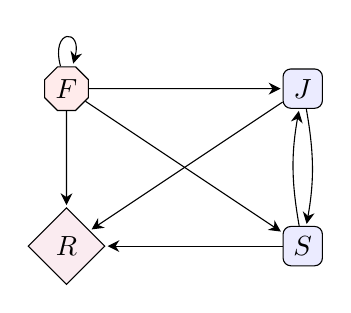
\begin{tikzpicture}[
  square/.style={rectangle, draw=black, minimum width=0.5cm, minimum height=0.5cm, rounded corners=.1cm, fill=blue!8},
  rhombus/.style={diamond, draw=black, minimum width=0.1cm, minimum height=0.1cm, fill=purple!8,aspect = 1},
  travel/.style={circle, draw=black, minimum width=0.5cm, minimum height=0.5cm, fill=green!8},
  report/.style={shape=regular polygon, regular polygon sides=8, draw, fill=red!8,minimum size=0.6cm,inner sep=0cm},
  bendy/.style={bend left=10},
  bendy2/.style={bend left=100},
  bendy3/.style={bend left=-100},
  >/.style={shorten >=0.25mm},
  >/.tip={Stealth[length=1.5mm,width=1.5mm]}
]
\tikzset{>={}};

\node (Sn) at (5.5,0) [square] {$S$};
\node (Jn) at (5.5,2) [square] {$J$};
\node (R) at (2.5,0)  [rhombus] {$R$};
\node (F) at (2.5,2) [report] {$F$};



\draw [->, bendy] (Jn) to  (Sn);
\draw [->, bendy] (Sn) to  (Jn);


\draw [->] (F) --  (R);
\draw [->] (Sn) -- (R);
\draw [->] (Jn) -- (R);
\draw [->] (F) -- (Sn);
\draw [->] (F) -- (Jn);
\draw (F) edge[loop above] (F);


\end{tikzpicture}
}
\end{center}
\vspace{-5mm}
\caption{Flow diagram for the SRJF model illustrating population interactions. The model includes the $R$ state, representing mortality. For $\species \in \{\native,\invasive\}$, susceptible populations ($S^{\species}$) can reproduce into juvenile ($J^{\species}$) and \textit{A.} Algae ($F$) will be refilled, as shown by the recycling arrows. Both $S^{\species}$ and $J^{\species}$ consume resources from $F$, and over time, components in $F$ also progress to $R$.}
\label{fig:SRJF}
\end{figure}

\begin{figure}[H]
\centering
\begin{knitrout}
\definecolor{shadecolor}{rgb}{0.969, 0.969, 0.969}\color{fgcolor}
\includegraphics[width=\textwidth]{figure/DataVisSRJFdent-1} 
\end{knitrout}
\caption{\label{fig:data_vis_SRJF_dent}
Density (Individuals$/$Liter) of \textit{D.~dentifera}.
The top panel shows adult susceptibles (\textit{D.~dentifera}, black).
The bottom panel shows juvenile susceptibles (\textit{D.~dentifera}, orange).
There were negligible infected juveniles.
Columns are buckets corresponding to replications with same treatment setting.
}
\end{figure}

\begin{figure}[H]
\centering
\begin{knitrout}
\definecolor{shadecolor}{rgb}{0.969, 0.969, 0.969}\color{fgcolor}
\includegraphics[width=\textwidth]{figure/DataVisSRJFlumdata-1} 
\end{knitrout}
\caption{\label{fig:data_vis_SIPJF_lum}
Density (Individuals$/$Liter) of \textit{D.~lumholtzi}.
The top panel shows adult susceptibles (\textit{D.~lumholtzi}, blue).
The bottom panel shows juvenile susceptibles (\textit{D.~lumholtzi}, purple).
There were negligible infected juveniles.
Columns are buckets corresponding to replications with same treatment setting.
}
\end{figure}

\subsection{Results}

\begin{table}[H]
\centering
\resizebox{\textwidth}{!}{
\begin{tabular}{||c|c |c|c|c||}
\hline
Parameter & Definition &Unit & Value & CI\\[0.5ex]
\hline
\hline
$S^{\native}$ & Susceptible host density   & $\mathrm{individual} \cdot L ^{-1}$                 & Variable                & \\
$J^{\native}$ & Juvenile host density    & $ \mathrm{individual} \cdot L ^{-1}$                & Variable                & \\
$F$   & Alga density                              & $10^6 \cdot \mathrm{cell} \cdot L ^{-1}$             & Variable                & \\
$r^{\native}$ &  Birth rate of juvenile                        & $\mathrm{individual} \cdot 10^{-6}\cdot \mathrm{cell}^{-1}$ & $1.69\cdot 10^{3}$  & ($6.78\cdot 10^{2}$,$4.53\cdot 10^{3}$)\\
$f^{\native}_{S}$ & Susceptible adult host filtering rate   &  $\mathrm{L} \cdot \mathrm{individual}^{-1} \cdot \mathrm{day}^{-1}$   & $1.32\cdot 10^{-4}$  & ($7.29\cdot 10^{-5}$,$2.39\cdot 10^{-4}$)\\
$r^{\native} \cdot f_{S^{\native}}$          & Effective Birth rate of native juvenile            &     $10^{-6} \cdot \mathrm{L} \cdot \mathrm{cell}^{-1} \cdot \mathrm{day}^{-1} $ & $2.23\cdot 10^{-1}$  & ($1.53\cdot 10^{-1}$,$3.59\cdot 10^{-1}$)\\
$\theta^{\native}_{S}$ & Susceptible adult host mortality rate     &     $  \mathrm{day}^{-1}$     & $6.92\cdot 10^{-1}$  & ($4.27\cdot 10^{-1}$,$1.27$)\\
$\theta^{\native}_{J}$ & Juvenile mortality rate        &     $ \mathrm{day}^{-1}$     & $2.13\cdot 10^{-8}$  & (0,$4.56\cdot 10^{-2}$)\\
$\lambda^{\native}_{J}$ & Maturation rate of the juvenile                  &     $ \mathrm{day}^{-1} $                  & $1.00\cdot 10^{-1}$  & \\
$\xi_J$         & Ratio of juvenile individual filtering rate &     $\mathrm{Unitless}$                    & $1.00$ & \\
$\beta^{\native}$       & Spores produced by death per infected individual     &  $10^3 \cdot \mathrm{spore} \cdot \mathrm{individual}^{-1} \cdot \mathrm{day}^{-1}$  & $3.00\cdot 10$ & \\
$\mu$           & Algae refilling rate                                &  $10^6 \cdot \mathrm{cell} \cdot \mathrm{L} ^{-1} \cdot \mathrm{day}^{-1}$                 & $3.70\cdot 10^{-1}$ & \\
$\delta$        & Sampling rate                                      &  $day ^{-1}$                                                                         & $1.30\cdot 10^{-2}$ & \\
$\sigma^{\native}_{S}$ & Standard deviation of Brownian motion of susceptible adult               &   $\sqrt{\mathrm{individual} \cdot \mathrm{day}^{-1}}$  & 0  & \\
$\sigma^{\native}_{J}$ & Standard deviation of Brownian motion of juvenile               &   $\sqrt{\mathrm{individual} \cdot \mathrm{day}^{-1}}$  & $3.07\cdot 10^{-1}$  & ($2.31\cdot 10^{-1}$,$3.81\cdot 10^{-1}$)\\
$\sigma_{F}$   & Standard deviation of Brownian motion of alga                          &   $\sqrt{\mathrm{individual} \cdot \mathrm{day}^{-1}}$  & $9.31\cdot 10^{-7}$  & (0,$4.60\cdot 10^{-2}$)\\
$\tau^{\native}_{S}$      &  Measurement dispersion for susceptible adult          &$\mathrm{Unitless}$           & $1.34\cdot 10$  & ($6.77$,$9.81\cdot 10$)\\
\hline
\end{tabular}}
\caption{Variables and parameter definitions and estimates of SRJF model for \textit{D.~dentifera}-only dynamics. The confidence interval is generated by the Monte Carlo Adjusted Profile.}
\label{Table:SRJF_native}
\end{table}


\begin{table}[H]
\centering
\resizebox{\textwidth}{!}{
\begin{tabular}{||c|c |c|c|c||}
\hline
Parameter & Definition &Unit & Value & CI\\[0.5ex]
\hline
\hline
$S^{\invasive}$ & Susceptible host density   & $\mathrm{individual} \cdot L ^{-1}$                 & Variable                & \\
$J^{\invasive}$ & Juvenile host density    & $ \mathrm{individual} \cdot L ^{-1}$                & Variable                & \\
$F$   & Alga density                              & $10^6 \cdot \mathrm{cell} \cdot L ^{-1}$             & Variable                & \\
$r^{\invasive}$ &  Birth rate of juvenile                        & $\mathrm{individual} \cdot 10^{-6}\cdot \mathrm{cell}^{-1}$ & $9.77\cdot 10^{2}$  & ($8.86\cdot 10$,$\infty$)\\
$f^{\invasive}_{S}$ & Susceptible adult host filtering rate   &  $\mathrm{L} \cdot \mathrm{individual}^{-1} \cdot \mathrm{day}^{-1}$   & $2.67\cdot 10^{-4}$  & (0,$1.34\cdot 10^{-3}$)\\
$r^{\invasive} \cdot f_{S^{\invasive}}$          & Effective Birth rate of invasive juvenile            &     $10^{-6} \cdot \mathrm{L} \cdot \mathrm{cell}^{-1} \cdot \mathrm{day}^{-1} $ & $2.61\cdot 10^{-1}$  & ($9.04\cdot 10^{-2}$,$4.02$)\\
$\theta^{\invasive}_{S}$ & Susceptible adult host mortality rate     &     $ \mathrm{day}^{-1}$     & $5.99\cdot 10^{-1}$  & ($2.26\cdot 10^{-1}$,$1.40$)\\
$\theta^{\invasive}_{J}$ & Juvenile mortality rate        &     $ \mathrm{day}^{-1}$     & $2.98\cdot 10^{-1}$  & (0,$4.58$)\\
$\lambda^{\invasive}_{J}$ & Maturation rate of the juvenile                  &     $ \mathrm{day}^{-1} $                  & $1.00\cdot 10^{-1}$  & \\
$\xi_J$         & Ratio of juvenile individual filtering rate &     $\mathrm{Unitless}$                    & $1.00$ & \\
$\beta^{\invasive}$       & Spores produced by death per infected individual     &  $10^3 \cdot \mathrm{spore} \cdot \mathrm{individual}^{-1} \cdot \mathrm{day}^{-1}$  & $3.00\cdot 10$ & \\
$\mu$           & Algae refilling rate                                &  $10^6 \cdot \mathrm{cell} \cdot \mathrm{L} ^{-1} \cdot \mathrm{day}^{-1}$                 & $3.70\cdot 10^{-1}$ & \\
$\delta$        & Sampling rate                                      &  $day ^{-1}$                                                                         & $1.30\cdot 10^{-2}$ & \\
$\sigma^{\invasive}_{S}$ & Standard deviation of Brownian motion of susceptible adult               &   $\sqrt{\mathrm{individual} \cdot \mathrm{day}^{-1}}$  & 0  & \\
$\sigma^{\invasive}_{J}$ & Standard deviation of Brownian motion of juvenile               &   $\sqrt{\mathrm{individual} \cdot \mathrm{day}^{-1}}$  & $3.78\cdot 10^{-1}$  & (0,$5.07\cdot 10^{-1}$)\\
$\sigma^{\invasive}_{F}$   & Standard deviation of Brownian motion of alga                          &   $\sqrt{\mathrm{individual} \cdot \mathrm{day}^{-1}}$  & $4.73\cdot 10^{-2}$  & (0,$1.38\cdot 10^{-1}$)\\
$\tau^{\invasive}_{S}$      &  Measurement dispersion for susceptible adult           &$\mathrm{Unitless}$           & $2.35$  & ($1.32$,$5.72$)\\
\hline
\end{tabular}}
\caption{Variables and parameter definitions and estimates of SRJF model for \textit{D.~lumholtzi}-only dynamics. The confidence interval is generated by the Monte Carlo Adjusted Profile.}
\label{Table:SRJF_invasive}
\end{table}

\begin{figure}[H]
    \centering
    \includegraphics[width=\linewidth]{profile/Simple_dynamics/Dent/no_para/Profile_plot.png}
    \caption{Monte Carlo Adjusted Profile results of SRJF model for \textit{D.~dentifera}-only dynamics.
    The vertical dotted lines represent the 95\% confidence interval obtained by MCAP.
    The vertical blue lines show the MLE estimated using MCAP.
    The red vertical lines correspond to the model with the overall highest likelihood among all searches.
}
    \label{fig:SRJF_dent_profile}
\end{figure}

\begin{figure}[H]
    \centering
    \includegraphics[width=\linewidth]{profile/Simple_dynamics/Lum/no_para/Profile_plot.png}
    \caption{Monte Carlo Adjusted Profile results of SRJF model for \textit{D.~lumholtzi}-only dynamics.
    The vertical dotted lines represent the 95\% confidence interval obtained by MCAP.
    The vertical blue lines show the MLE estimated using MCAP.
    The red vertical lines correspond to the model with the overall highest likelihood among all searches.
}
    \label{fig:SRJF_lum_profile}
\end{figure}

\begin{table}[h!]
\centering
\begin{center}
\begin{tabular}{||c |c |c |c|c|c||}
 \hline
Specific parameters  & Max log-likelihood & AIC & \makecell[c]{Max log-likelihood\\(block)} & \makecell[c]{AIC\\(block)} & \makecell[c]{LRT\\$p$-value}\\ [0.5ex]
 \hline\hline
$\varnothing$ & -498.78& 1011.56& -498.78& 1011.56 & --- \\
$\theta^{\native}_{S,\unit}$  & -490.57& 1013.14& -489.85& 1011.71 & 0.06 \\
$r^{\native}_{\unit}$ & -497.43& 1026.85& -496.44& 1024.89 & 0.97 \\
$f^{\native}_{S,\unit}$ & -497.43& 1026.86& -496.16& 1024.32 & 0.98\\[1ex]
 \hline
\end{tabular}
\end{center}
\caption{Comparison of model fit and complexity across various configurations of unit-specific parameters within the panelPOMP framework for \textit{D.~dentifera}-only dynamics. The unit-specific parameter setting assessed include $f^{\native}_{S,\unit}$, $r^{\native}_{\unit}$, $\theta^{\native}_{S,\unit}$.}
\label{Table:SRJF_dent_model_comparison}
\end{table}

\begin{table}[h!]
\centering
\begin{center}
\begin{tabular}{||c |c |c |c|c|c||}
 \hline
Specific parameters  & Max log-likelihood & AIC & \makecell[c]{Max log-likelihood\\(block)} & \makecell[c]{AIC\\(block)} & \makecell[c]{LRT\\$p$-value}\\ [0.5ex]
 \hline\hline
$\varnothing$ & -372.15& 758.294& -372.15& 758.294 & --- \\
$\theta^{\invasive}_{S,\unit}$  & -365.33& 762.658& -365.37& 762.733 & 0.14 \\
$r^{\invasive}_{\unit}$ & -366.84& 765.676& -366.29& 764.571 & 0.30 \\
$f^{\invasive}_{S,\unit}$ & -368.15& 768.300& -368.07& 768.147 & 0.53 \\[1ex]
 \hline
\end{tabular}
\end{center}
\caption{Comparison of model fit and complexity across various configurations of unit-specific parameters within the panelPOMP framework for \textit{D.~lumholtzi}-only dynamics. The unit-specific parameter setting assessed include $f^{\invasive}_{S,\unit}$, $r^{\invasive}_{\unit}$, $\theta^{\invasive}_{S,\unit}$.}
\label{Table:SRJF_lum_model_comparison}
\end{table}

The data plots, parameter estimates, and profile likelihood plots are analogous to the results in the main text, applied here to the SRJF model for either \textit{D.~dentifera} or \textit{D.~lumholtzi}.

The results in Tables~\ref{Table:SRJF_dent_model_comparison} and~\ref{Table:SRJF_lum_model_comparison} indicate that the model configuration with all shared parameters achieves the minimum AIC score for both dynamics, suggesting that this model makes a successful balance between model fit and complexity.
The LRT $p$-values further support this choice, as none of the unit-specific models show a statistically significant improvement over the all-shared baseline.
These results are consistent with our other analysis.

\subsection{Simulation}
The simulation plots (Figures \ref{fig:SRJF_native_simulation_band} to \ref{fig:SRJF_lum_simulation_lines}) collectively demonstrate the SRPF model's capability to capture the complex interactions among various states within the population dynamics of \textit{D.~dentifera} and \textit{D.~lumholtzi}.
Specifically, the model effectively reproduces the latent patterns for susceptible and infected densities across multiple experimental units, as evidenced by the close alignment between the simulated mean trajectories (depicted by the black and light-blue bands) and the observed experimental data (represented by colorful solid lines).
Each blue line illustrates an individual simulation case, capturing the stochastic variability across replicates, while the light blue shaded area (where present) denotes the 95\% confidence interval of the simulation results.
Although juvenile density data were not included in the model fitting process, the model still accurately predicts juvenile density trends (Figures \ref{fig:SRJF_lum_simulation_lines}).
This performance indicates the model's capacity to generalize underlying ecological processes, as the 95\% confidence intervals largely encompass the observed juvenile data.
The model also predicts a decline in algal density as the experiment progresses.
This predicted reduction in food availability provides a mechanistic explanation for the observed trends in \textit{Daphnia} densities, as resource scarcity constrains population growth, ultimately affecting the susceptible, infected, and juvenile densities.


\begin{figure}[H]
    \centering
    \includegraphics[width=0.75\linewidth]{simulation/dent_no_para_simulation/simulation_band.png}
    \caption{Simulation plots of densities (Individuals$/$Liter) for susceptible, and juvenile \textit{D.~dentifera}, along with alga density ($10^6\,$cells$/$Liter) and parasite density  ($10^3\,$spores$/$Liter), over time (days). The colorful solid lines represent observed experimental data, showing the variability across different experimental replicates. The black line represents the mean trajectory from the simulation model, capturing the general trend of each density. The light blue shaded area corresponds to the 95\% confidence interval of the simulations, indicating the range of model predictions. Dashed lines illustrate individual simulated trajectories, highlighting the model’s ability to capture fluctuations around the mean trajectory.}
    \label{fig:SRJF_native_simulation_band}
\end{figure}


\begin{figure}[H]
    \centering
    \includegraphics[width=0.75\linewidth]{simulation/dent_no_para_simulation/simulation_lines.png}
   \caption{Simulated densities (Individuals$/$Liter) of susceptible \textit{D.~dentifera}, juvenile \textit{D.~dentifera} and alga density ($10^6\,$cells$/$Liter) over time (days) for each experimental unit. The blue lines represent individual simulation runs, capturing the variability in susceptible density across replicates, while the red line represents the actual experiment data.}
    \label{fig:SRJF_dent_simulation_lines}
\end{figure}


\begin{figure}[H]
    \centering
    \includegraphics[width=0.75\linewidth]{simulation/lum_no_para_simulation/simulation_band.png}
    \caption{Simulation plots of densities (Individuals$/$Liter) for susceptible, and juvenile \textit{D.~lumholtzi}, along with alga density ($10^6\cdot$cells$/$Liter) and parasite density  ($10^3\cdot$spores$/$Liter), over time (days). The colorful solid lines represent observed experimental data, showing the variability across different experimental replicates. The black line represents the mean trajectory from the simulation model, capturing the general trend of each density. The light blue shaded area corresponds to the 95\% confidence interval of the simulations, indicating the range of model predictions. Dashed lines illustrate individual simulated trajectories, highlighting the model’s ability to capture fluctuations around the mean trajectory.}
    \label{fig:SRJF_invasive_simulation_band}
\end{figure}

\begin{figure}[H]
    \centering
    \includegraphics[width=0.75\linewidth]{simulation/lum_no_para_simulation/simulation_lines.png}
   \caption{Simulated densities (Individuals$/$Liter) of susceptible \textit{D.~lumholtzi} and juvenile \textit{D.~lumholtzi},  with  alga density ($10^6\cdot$cells$/$Liter), for each experimental unit. The blue lines represent individual simulation runs, capturing the variability in susceptible density across replicates, while the red line represents the actual experiment data.}
    \label{fig:SRJF_lum_simulation_lines}
\end{figure}

\section{Benchmark Models}
\subsection{Searle et al.’s Model}

Using the mechanistic model introduced by \citet{searle16}, we conduct predictions of population $\tilde{y}_{\unit,\benchmarktime}$ for susceptible, infected \textit{D.~dentifera} and \textit{D.~lumholtzi} for all time $\benchmarktime \in \{1,2,\dots,N_{\unit}\}$ and units $\unit \in \{1,2,\dots,U\}$.
In our case, each unit is observed at the same number of time points, so $N_{\unit} = N$ for all $\unit$.
Then, we obtain the overall log-likelihood by summing the log-probabilities of the observed density of \textit{Daphnia}.
Specifically, we use the observed densities $y^*_{\unit,\benchmarktime}$ and the predicted means $\tilde{y}_{\unit,\benchmarktime}$ derived from the mechanistic model, along with the dispersion parameter $\tau$ to specify a NBinom distribution and calculate the likelihood:
\begin{align}
\ell(\beta, \theta) &= \sum_{\unit=1}^{\Unit}\sum_{\benchmarktime=1}^{N}
\log P(Y_{\unit,\benchmarktime} = y^*_{\unit,\benchmarktime} \mid \mu_{\unit,\benchmarktime}, \tau),
\label{eq:total_loglik}
\end{align}

To obtain the maximum likelihood estimate, we conduct the linear optimization on $\tau$ and choose the $\hat{\tau}$ that yields the highest overall likelihood. 
With this $\hat{\tau}$, we obtain the likelihood by \ref{eq:total_loglik} for the model on the data. And the result of the model fitting can be found in the Table~2 in the main article.

\subsection{Negative Binomial Regression}

Count data from ecological studies often exhibit overdispersion and unit-specific variation.
The NBinom distribution addresses overdispersion, while random intercepts allow each unit to have its own baseline level.
As a benchmark model, we employ NBinom generalized linear mixed models (GLMMs) to capture overdispersed count data and correlation across repeated measures within each unit $\unit$.
The NBinom distribution is parameterized by a mean $\mu_{\unit,\benchmarktime}$ and a dispersion parameter $\theta$.

We present three GLMMs with increasing of order of time factor to capture the trend of these \textit{Daphnia} species in the experiment.
While a linear model is easy to interpret and straightforward to implementing, observed \textit{Daphnia} data exhibit a non-linear pattern.
Introducing quadratic or cubic terms to the model enhance the capability of model to capture these non-linear trends in the data.
By starting with a linear model and then considering quadratic and cubic cases, we can evaluate the complexity of temporal patterns and better approximate the latent process of in the dynamics.

\subsubsection{Model 1 (Linear Trend Model)}
We start with a simple GLMM having only with linear terms:
\begin{align}
Y_{\unit,\benchmarktime} &\sim \text{NBinom}(\mu_{\unit,\benchmarktime}, \tau), \\[6pt]
\log(\mu_{\unit,\benchmarktime}) &= \beta_0 + \beta_1\, t_{\unit,\benchmarktime} + b_{\unit},
\label{model:GLMM_linear}
\end{align}
where $\mu_{\unit,\benchmarktime}$ is the expected count for unit $\unit$ at time $\benchmarktime$.
We fit this model independently for each {\it Daphnia} species, life stage, and infection status, and so the total log-likelihood is the sum over these categories.
The vector coefficient $\beta_1$ measures the effect of time on the log-scale of \textit{Daphnia} density.
The term $b_\unit$ accounts for the random intercept drawn from a normal distribution with variance $\sigma^2$.
Conditional on the random intercept $b_\unit$, observations within a unit are assumed independent.
The dispersion parameter $\tau$ from the NBinom distribution accommodates overdispersion in the count data, which is density in our case.


\subsubsection{Model 2 (Quadratic Trend Model)}
To accommodate the non-linear pattern, we include a quadratic term in time in model~\ref{model:GLMM_quad}:
\begin{align}
Y_{\unit,\benchmarktime} &\sim \text{NBinom}(\mu_{\unit,\benchmarktime}, \tau), \\[6pt]
\log(\mu_{\unit,\benchmarktime}) &= \beta_0 + \beta_1\, t_{\unit,\benchmarktime} + \beta_2\, t_{\unit,\benchmarktime}^2 + b_{\unit}.
\label{model:GLMM_quad}
\end{align}
Here, $\beta_2$ captures curvature in the trend, allowing for a turning point as time progresses.

\subsubsection{Model 3 (Cubic Trend Model)}
To capture more complex temporal pattern, we further introduce the cubic term in the model~\ref{model:GLMM_cubic}:
\begin{align}
Y_{\unit,\benchmarktime} &\sim \text{NBinom}(\mu_{\unit,\benchmarktime}, \tau), \\[6pt]
\log(\mu_{\unit,\benchmarktime}) &= \beta_0 + \beta_1\, t_{\unit,\benchmarktime} + \beta_2\, t_{\unit,\benchmarktime}^2 + \beta_3\, t_{\unit,\benchmarktime}^3 + b_{\unit}.
\label{model:GLMM_cubic}
\end{align}
The cubic term $\beta_3$ provides additional capability for capturing multiple fluctuation patterns in the \textit{Daphnia} dynamics.


The likelihood for these models is constructed by considering the joint distribution of all observations $\{Y_{u,n}\}$, integrating over the random effects, $b_{1:\Unit}$. Letting $\beta = (\beta_0, \beta_1, \dots)$ denote the fixed-effect parameters, the conditional likelihood of the observations for unit $\unit$ given $b_\unit$ is
\begin{align}
L_\unit(\beta, \tau, \sigma^2) &= \prod_{\benchmarktime=1}^{N} f_{\text{NB}}\bigl(Y_{\unit,\benchmarktime}; \mu_{\unit,\benchmarktime}(\beta, \sigma^2), \tau\bigr),
\label{eq:conditional_likelihood}
\end{align}
where $f_{\text{NB}}(\cdot;\mu,\tau)$ is the NBinom probability mass function and $\mu_{\unit,\benchmarktime}(\beta, b_\unit) = \exp(\beta_0 + \beta_1 t_{\unit,\benchmarktime} + \dots + b_\unit)$. 
The total likelihood is then the product over all units due to the independence:
\begin{align}
L(\beta, \tau, \sigma^2) &= \prod_{\unit=1}^{\Unit} L_\unit(\beta, \tau, \sigma^2)\\
                         &= \prod_{\unit=1}^{\Unit} \prod_{\benchmarktime=1}^{N} f_{\text{NB}}\bigl(Y_{\unit,\benchmarktime}; \mu_{\unit,\benchmarktime}(\beta, \sigma^2), \tau\bigr)
\label{eq:total_likelihood}
\end{align}
and the log-likelihood is:
\begin{align}
\ell(\beta, \tau, \sigma^2) &= \sum_{\unit=1}^{\Unit} \sum_{\benchmarktime=1}^{N} \log \bigl(f_{\text{NB}}(Y_{\unit,\benchmarktime}; \mu_{i,j}(\beta, \sigma^2), \tau)\bigl).
\label{eq:log_likelihood}
\end{align}
The calculated log-likelihood used to compute the AIC for model comparison. And the result of the model fitting of model~\ref{model:GLMM_linear},~\ref{model:GLMM_quad} and \ref{model:GLMM_cubic} can be found in the Table~2 in the main article.

\subsection{SIRPF2 Model}

The SIRPF2 model presented here ignores the state of juvenile \textit{Daphnia} and describes the dynamics in each bucket ($\unit$) among susceptible individuals ($S^{\species}$), infected individuals ($I^{\species}$), alga as a food resource ($F$), the parasite population ($P$).
The superscript $\species$ denotes the species, which represents native or invasive species.
Each stochastic differential equation accounts for various biological and ecological processes, augmented with stochastic terms to capture the inherent randomness within the systems.
{\small
\begin{align}
    dS^{\species}_{\unit}(t) &= r^{\species}_{\unit} \, f^{\species}_{S,{\unit}} \, F_{\unit}(t) \, S^{\species}_{\unit}(t)\, dt -
    \big\{
    \theta^{\species}_{S,{\unit}} + p^{\species}_{\unit} \, f^{\species}_{S,{\unit}} \, P_{\unit}(t) + \delta
    \big\}
    \, S^{\species}_{\unit}(t)\, dt,\\
    dI^{\species}_{\unit}(t) &= p^{\species}_{\unit} \, f^{\species}_{S,{\unit}}\,  S^{\species}_{\unit}(t) \, P_{\unit}(t)\, dt -
    \big\{
    \theta^{\species}_{I,{\unit}} + \delta
    \big\}
    \, I^{\species}_{\unit}(t)\, dt + I^{\species}_{\unit}(t) \, d\zeta^{\species}_{I,{\unit}},\label{eq:SIRPF2_dS}\\
    dP_{\unit}(t) &= \sum_{\species \in \{\native, \invasive\}} \left(\beta^{\species}_{\unit} \, \theta^{\species}_{I,{\unit}} \,  I^{\species}_{\unit}(t) - f^{\species}_{S,{\unit}} \big\{ S^{\species}_{\unit}(t) + \xi_{\unit} I^{\species}_{\unit}(t) \big\} P_{\unit}(t)\right) dt
    \\ \nonumber
    & \hspace{5cm} - \theta_{P,{\unit}} \, P_{\unit}(t)\, dt + P_{\unit}(t)\, d\zeta_{P,{\unit}},\\
    dF_{\unit}(t) &= - \sum_{\species \in \{\native, \invasive\}} f^{\species}_{S,{\unit}} \, F_{\unit}(t) \left(S^{\species}_{\unit}(t)+\xi_{\unit} \, I^{\species}_{\unit}(t)\right)dt  + \mu \, dt + F_{\unit}(t)\, d\zeta_{F,{\unit}},\label{eq:SIRPF2_dF}\\
d\zeta^{\species}_{I,{\unit}} &\sim \Normal \big[0, (\sigma^{\species}_{I,{\unit}})^{2}\, dt\big],
\hspace{5mm}
d\zeta_{F,{\unit}} \sim \Normal \big[0, \sigma_{F,{\unit}}^{2}\, dt\big],
\hspace{5mm}
d\zeta_{P,{\unit}} \sim \Normal \big[0, \sigma_{P,{\unit}}^{2}\, dt\big].
\end{align}
}


Unlike the SIRJPF2 model, we ignore the maturation process from juvenile to adult in equation \eqref{eq:SIRPF2_dS}.
Instead, this model uses $r^{\species}_{\unit}$ to represent the average rate of growth in density of \textit{Daphnia} adult.

\subsubsection{Flow Diagram}
The SIRPF2 model illustrates the interdependent dynamics among the Susceptible ($S$), Infected ($I$), Food ($F$), and Parasite ($P$) populations, with transitions representing ecological and biological interactions.

\usetikzlibrary{positioning}
\usetikzlibrary {arrows.meta}
\usetikzlibrary{shapes.geometric}

\begin{figure}[H]
\begin{center}
\resizebox{8cm}{!}{
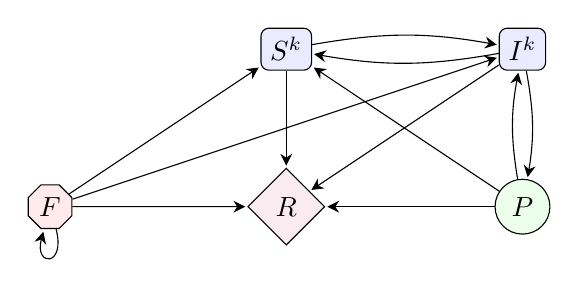
\begin{tikzpicture}[
  square/.style={rectangle, draw=black, minimum width=0.5cm, minimum height=0.5cm, rounded corners=.1cm, fill=blue!8},
  rhombus/.style={diamond, draw=black, minimum width=0.1cm, minimum height=0.1cm, fill=purple!8,aspect = 1},
  travel/.style={circle, draw=black, minimum width=0.5cm, minimum height=0.5cm, fill=green!8},
  report/.style={shape=regular polygon, regular polygon sides=8, draw, fill=red!8,minimum size=0.6cm,inner sep=0cm},
  bendy/.style={bend left=10},
  bendy2/.style={bend left=100},
  bendy3/.style={bend left=-100},
  >/.style={shorten >=0.25mm},
  >/.tip={Stealth[length=1.5mm,width=1.5mm]}
]
\tikzset{>={}};

\node (S) at (2.5,0) [square] {$S^{\species}$};
\node (I) at (5.5,0) [square] {$I^{\species}$};
\node (R) at (2.5,-2)  [rhombus] {$R$};
\node (P) at (5.5,-2)[travel] {$P$};
\node (F) at (-0.5,-2) [report] {$F$};



\draw [->, bendy] (S) to  (I);
\draw [->, bendy] (I) to  (S);


\draw [->] (P) --  (S);
\draw [->] (F) --  (R);
\draw [->] (P) --  (R);
\draw [->] (S) -- (R);
\draw [->] (I) -- (R);
\draw [->] (F) -- (S);
\draw [->] (F) -- (I);
\draw (F) edge[loop below] (F);

\draw [->, bendy] (P) to (I);
\draw [->, bendy] (I) to (P);


\end{tikzpicture}
}
\end{center}
\vspace{-5mm}
\caption{Flow diagram for the SIRPF2 model illustrating population interactions.}
\label{fig:flow_SIRPF2}
\end{figure}

\section{Experimental Data on Peak Density}
\begin{table}[H]
\centering
\begin{tabular}{lccccc}
\toprule
Mesocosm
& \shortstack{\textit{D.~dentifera} \\ juvenile} 
& \shortstack{\textit{D.~dentifera} \\ female adult} 
& \shortstack{\textit{D.~lumholtzi} \\ juvenile} 
& \shortstack{\textit{D.~lumholtzi} \\ female adult} 
& \shortstack{\textit{D.~lumholtzi} \\ male adult} \\
\midrule
1 & 22 & 22 & 22 & 27 & 27 \\
2 & 22 & 32 & 17 & 17 & 22 \\
3 & 27 & 32 & 27 & 22 & 37 \\
4 & 22 & 22 & 37 & 17 & 27 \\
5 & 22 & 22 & 17 & 32 & 27 \\
6 & 32 & 27 & 27 & 32 & 42 \\
7 & 27 & 22 & 17 & 17 & 27 \\
8 & 27 & 32 & 22 & 22 & 42 \\
\bottomrule
\end{tabular}
\caption{This table shows the day on which each species reached its peak density in mesocosms containing both \textit{Daphnia} species and the parasite. \textit{D.~dentifera} male adults are excluded because they were almost absent.} \label{table:peak_density}
\end{table}

Table~\ref{table:peak_density} provides supporting data on the relative timing of peak abundance for different demographic groups.

\section{SIRJPF2-Gamma Model}
The SIRJPF2-Gamma model differs from the original SIRJPF2 model by its incorporation of gamma noise in transition processes between states, in place of the Gaussian noise used previously. 
Specifically, in the SIRJPF2-Gamma model, random fluctuations for transitions between states are explained by gamma distributions to represent ecological events occur through one-way transitions which are nonnegative. 
The use of gamma noise in modeling transitions explicitly enforces that individuals move from one class to another without the artificial creation or destruction of hosts that do not transit to or from another compartment.
This aligns with the underlying dynamics that the jump-like transitions observed in ecosystem reflect one-directional movements rather than symmetrical fluctuations.




{\small
\begin{align}
    dS^{\species}_{\unit}(t) &= \lambda^{\species}_{J,{\unit}} \,  J^{\species}_{\unit}(t)dt -
    \big\{
    \theta^{\species}_{S,{\unit}} + \delta
    \big\}
    \, S^{\species}_{\unit}(t)\, dt - p^{\species}_{\unit} \, f^{\species}_{S,{\unit}} \, P_{\unit}(t) S^{\species}_{\unit}(t) \, d\Gamma^{\species}_{SI,{\unit}},\\
    dI^{\species}_{\unit}(t) &= p^{\species}_{\unit} \, f^{\species}_{S,{\unit}}\,  S^{\species}_{\unit}(t) \, P_{\unit}(t)\, d\Gamma^{\species}_{SI,{\unit}} -
    \theta^{\species}_{I,{\unit}} I^{\species}_{\unit}(t)d\Gamma^{\species}_{IP,{\unit}}- \delta\, I^{\species}_{\unit}(t)\, dt,\\
    dJ^{\species}_{\unit}(t) &= r^{\species}_{\unit} \, f^{\species}_{S,{\unit}} \, F_{\unit}(t) \, S^{\species}_{\unit}(t)\, d\Gamma^{\species}_{SJ,{\unit}} -
    \big\{
    \theta^{\species}_{J,{\unit}}  + \delta
    \big\} 
    \, J^{\species}_{\unit}(t)\, dt - \lambda^{\species}_{J,{\unit}} \,  J^{\species}_{\unit}(t)dt, \\
    dP_{\unit}(t) &= \sum_{\species \in \{\native, \invasive\}} \left(\beta^{\species}_{\unit} \, \theta^{\species}_{I,{\unit}} \,  I^{\species}_{\unit}(t)d\Gamma^{\species}_{IP,{\unit}} - f^{\species}_{S,{\unit}} \big\{ S^{\species}_{\unit}(t) + \xi_{\unit} I^{\species}_{\unit}(t) \big\} P_{\unit}(t)dt\right) 
    \\ \nonumber & \hspace{7cm}
    - \theta_{P,{\unit}} \, P_{\unit}(t)\, dt,\\
    dF_{\unit}(t) &= - \sum_{\species \in \{\native, \invasive\}} f^{\species}_{S,{\unit}} \, F_{\unit}(t) \left(S^{\species}_{\unit}(t)+\xi_{J,{\unit}} \, J^{\species}_{\unit}(t) +\xi_{\unit} \, I^{\species}_{\unit}(t)\right)dt  + \mu \, dt + F_{\unit}(t)\, d\Gamma_{F,{\unit}},\\
d\Gamma^{\species}_{JS,{\unit}} &\sim \Gamma
  \bigg[\frac{dt}{(\sigma^{\species}_{JS,{\unit}})^{2}}, (\sigma^{\species}_{JS,{\unit}})^{2}\bigg],
\quad
d\Gamma^{\species}_{SI,{\unit}} \sim \Gamma
  \bigg[\frac{dt}{(\sigma^{\species}_{SI,{\unit}})^{2}}, (\sigma^{\species}_{SI,{\unit}})^{2}\bigg],\\
d\Gamma^{\species}_{IP,{\unit}} &\sim \Gamma
  \bigg[\frac{dt}{(\sigma^{\species}_{IP,{\unit}})^{2}}, (\sigma^{\species}_{IP,{\unit}})^{2}\bigg],
\quad
d\Gamma_{F,{\unit}} \sim \Normal \big[0, \sigma_{F,{\unit}}^{2}\, dt\big].
\end{align}
}
\bibliography{../bib-daphnia}
\end{document}
